\documentclass[11pt,a4paper]{article}

% ---------- codificación e idioma ----------
\usepackage[utf8]{inputenc}
\usepackage[T1]{fontenc}
\usepackage{lmodern}
\usepackage[spanish,es-tabla]{babel}
\usepackage{microtype}

% ---------- formato ----------
\usepackage[a4paper,margin=2.5cm]{geometry}
\usepackage{setspace}
\usepackage{fancyhdr}
\usepackage[section]{placeins}
\usepackage{enumitem}
\setlist{itemsep=2pt,topsep=4pt}

% ---------- figuras, tablas y unidades ----------
\usepackage{graphicx}
\usepackage{float}
\usepackage{booktabs}
\usepackage{tabularx}
\usepackage{array}
\usepackage{xcolor}
\usepackage{caption}
\usepackage{amsmath}
\usepackage{siunitx}
\sisetup{output-decimal-marker={,},group-separator={\,},group-minimum-digits=4}
\captionsetup{font=small,labelfont=bf,labelsep=period}

% ---------- código ----------
\usepackage{listings}
\definecolor{codegray}{gray}{0.45}
\lstdefinestyle{vhdlstyle}{
  basicstyle=\ttfamily\footnotesize,
  keywordstyle=\color{blue!60!black}\bfseries,
  commentstyle=\color{codegray}\itshape,
  numbers=left,numberstyle=\tiny\color{codegray},
  breaklines=true,frame=single,
  language=VHDL,
  extendedchars=true,
  literate={á}{{\'a}}1 {é}{{\'e}}1 {í}{{\'i}}1 {ó}{{\'o}}1 {ú}{{\'u}}1
           {ñ}{{\~n}}1 {Á}{{\'A}}1 {É}{{\'E}}1 {Í}{{\'I}}1 {Ó}{{\'O}}1 {Ú}{{\'U}}1
           {ü}{{\"u}}1 {¿}{{?`}}1 {¡}{{!`}}1
}
\lstdefinestyle{xdcstyle}{
  basicstyle=\ttfamily\footnotesize,
  commentstyle=\color{codegray}\itshape,
  morecomment=[l]{\#},
  breaklines=true,frame=single
}

% ---------- enlaces ----------
\usepackage[hidelinks]{hyperref}

% ---------- macros ----------
\newcommand{\code}[1]{\texttt{\detokenize{#1}}}
\newcommand{\todo}[1]{\colorbox{yellow}{\textit{[COMPLETAR: #1]}}}
\newcommand{\todoblock}[1]{\par\noindent\colorbox{yellow}{\parbox{\dimexpr\linewidth-2\fboxsep\relax}{\textit{[COMPLETAR: #1]}}}\par}
\newcommand{\placeholderfig}[2]{%
  \begin{figure}[H]
    \centering
    \fbox{\parbox{0.9\linewidth}{\centering\vspace{1.2em}%
      \colorbox{yellow}{\parbox{0.8\linewidth}{\centering\textit{[INSERTAR CAPTURA: #1]}}}%
      \vspace{1.2em}}}
    \caption{#2}
  \end{figure}}

% ---------- encabezado y pie ----------
\pagestyle{fancy}
\fancyhf{}
\fancyhead[L]{\small Modulador PPM controlado por UART en FPGA}
\fancyhead[R]{\small Circuitos Lógicos Programables -- CESE}
\fancyfoot[C]{\thepage}
\renewcommand{\headrulewidth}{0.4pt}

\onehalfspacing
\setlength{\emergencystretch}{2em}

\begin{document}

% =============================== PORTADA ===============================
\begin{titlepage}
\centering

\includegraphics[width=0.55\linewidth]{fig/logo_fiuba.png}\par
\vspace{1.5cm}
{\large Especialización en Sistemas Embebidos\par}
\vspace{0.4cm}
{\Large\bfseries Circuitos Lógicos Programables\par}
\vspace{0.4cm}
{\Large Trabajo práctico final\par}
\vspace{2.2cm}
\hrule
\vspace{0.6cm}
{\huge\bfseries Modulador PPM controlado por UART\\[0.3cm] implementado en FPGA\par}
\vspace{0.6cm}
\hrule
%\vfill
\vspace{0.7cm}
{\large Alumno: Mauro Ariel Gianchino\par}
\vspace{0.3cm}
{\large Fecha: 13/10/2026\par}
\end{titlepage}

\pagestyle{fancy}
\setcounter{page}{1}

% =============================== RESUMEN ===============================
\begin{abstract}
\noindent
Se presenta la implementación en una FPGA de un modulador por posición de pulso (PPM) descripto en VHDL.
El sistema recibe bytes por un puerto UART y, por cada uno, genera un único pulso cuya posición dentro de
una trama periódica de \SI{2,56}{\milli\second} codifica su valor (0 a 255), junto con una señal de
sincronismo que marca el comienzo de cada trama. El diseño se simuló con ModelSim, se sintetizó e
implementó con Vivado para la placa Arty Z7-10 y se verificó en hardware con un analizador lógico.
\end{abstract}

{\singlespacing\tableofcontents}
\newpage

% =============================== 1. INTRODUCCION ===============================
\section{Introducción y objetivo}

Este trabajo implementa en una FPGA un modulador PPM (\emph{Pulse Position Modulation}) descripto en VHDL.
El sistema recibe bytes por un puerto UART y, por cada byte recibido, genera un único pulso cuya posición
dentro de una trama periódica codifica el valor del byte. Una segunda salida marca el comienzo de cada trama
y sirve de referencia de tiempo para medir la posición del pulso.

El diseño se simuló con ModelSim, se sintetizó e implementó con Vivado 2018.3 para la placa Digilent
Arty Z7-10, y se verificó en hardware con un analizador lógico, enviando caracteres desde una PC a través de
un adaptador USB-serie.

% =============================== 2. PPM ===============================
\section{Modulación por posición de pulso}

En la modulación PPM la información no se codifica en la amplitud ni en el ancho del pulso, que son siempre los mismos, sino en la posición temporal en que este aparece. Para ello se divide el tiempo en tramas de duración $T$, y cada trama en $M$ ranuras iguales de duración $\tau$; el dato $d$ determina en cuál de ellas se coloca el pulso. La duración de la trama resulta entonces

\begin{equation}
  T = M\,\tau .
\end{equation}

El dato $d \in \{0, 1, \dots, M-1\}$ determina la ranura en la que se coloca el pulso, es decir, su posición dentro de la trama medida desde el inicio:

\begin{equation}
  t_d = d\,\tau .
\end{equation}


% =============================== 3. SISTEMA ===============================
\section{Descripción del sistema}

\subsection{Parámetros de diseño}

\begin{table}[H]
\centering
\small
\renewcommand{\arraystretch}{0.9}
\caption{Parámetros del diseño.}
\label{tab:parametros}
\begin{tabularx}{\linewidth}{@{}l X@{}}
\toprule
\textbf{Parámetro} & \textbf{Valor} \\
\midrule
Placa / FPGA & Digilent Arty Z7-10 \\
Frecuencia de clock & \SI{125}{\mega\hertz}; período de \SI{8}{\nano\second} \\
Duración de la ranura $\tau$ (= ancho del pulso) & \SI{10}{\micro\second} = 1250 ciclos de clock \\
Cantidad de ranuras $M$ & 256: una por cada valor de un byte (0 a 255) \\
Trama $T$ & $256 \times \SI{10}{\micro\second} = \SI{2,56}{\milli\second} = \num{320000}$ ciclos (390 tramas por segundo) \\
Pulso de sincronismo & \SI{1}{\micro\second} = 125 ciclos, al comienzo de cada trama \\
UART & \num{115200} baudios, 8N1 \\
Posición del pulso para el dato $d$ &  $ d \times \tau $ \\
\bottomrule
\end{tabularx}
\end{table}

Se eligió \SI{10}{\micro\second} como resolución temporal ya que equivale a 240 muestras de un analizador
lógico de \SI{24}{\mega\hertz}, lo que permite medir la posición con facilidad. Los criterios de diseño adoptados son:

\begin{itemize}
  \item \textbf{Un pulso por byte.} Si al comenzar una trama no hay un byte nuevo esperando, la trama va vacía (sin pulso).
  \item \textbf{Byte previo al inicio de trama.} El byte recibido durante una trama se guarda y recién se usa en la trama siguiente, de modo que ninguna trama tenga un pulso a medias ni dos pulsos.
  \item \textbf{El primero gana.} Si llegan varios bytes durante una trama, se modula el primero y se descartan los demás.
  \item \textbf{Sin ranura de seguridad.} El byte 255 usa la última ranura. Si en tramas consecutivas se usaran el 255 y el 0, los dos pulsos quedarían pegados y se verían como uno solo.
\end{itemize}

\subsection{Interfaz}

El sistema se presenta como un único módulo, \code{uart_top}, con cinco puertos (figura~\ref{fig:cajanegra}).
Recibe tres señales externas: el clock de \SI{125}{\mega\hertz} de la placa, un reset manual y la línea serie
del UART por la que llegan los bytes a modular. Entrega dos salidas: \code{ppm_pin}, con el pulso cuya posición
codifica el byte recibido, y \code{sync_pin}, que marca el comienzo de cada trama y sirve de referencia para
medir esa posición. En la tabla~\ref{tab:pines} se indica la función de cada puerto y el pin de la FPGA al que
está asignado.

\begin{figure}[H]
  \centering
  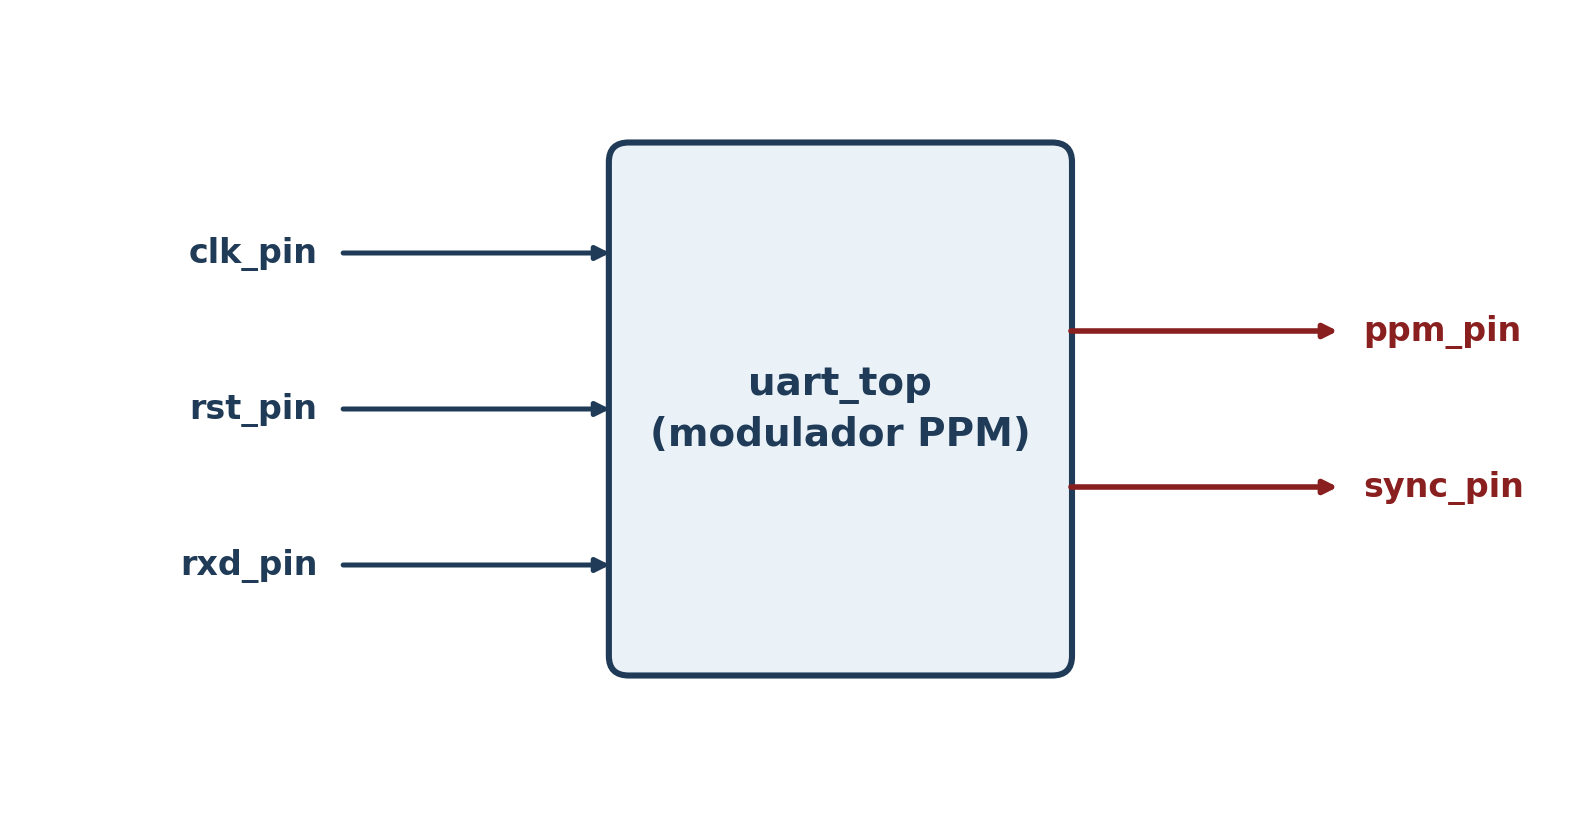
\includegraphics[width=0.8\linewidth]{fig/caja_negra_top.png}
  \caption{Módulo \code{uart_top}.}
  \label{fig:cajanegra}
\end{figure}

\begin{table}[H]
\centering
\small
\renewcommand{\arraystretch}{0.9}
\caption{Puertos del top y asignación de pines.}
\label{tab:pines}
\begin{tabular}{@{}l l l l@{}}
\toprule
\textbf{Puerto} & \textbf{I/O} & \textbf{Pin} & \textbf{Descripción} \\
\midrule
\code{clk_pin}  & Entrada & H16                  & Clock de \SI{125}{\mega\hertz} \\
\code{rst_pin}  & Entrada & L19 (BTN3)           & Reset activo en alto \\
\code{rxd_pin}  & Entrada & Y18 (PMOD JA, pin 1) & Entrada UART \\
\code{ppm_pin}  & Salida  & Y16 (PMOD JA, pin 3) & Salida PPM \\
\code{sync_pin} & Salida  & Y17 (PMOD JA, pin 4) & Sincronización \\
\bottomrule
\end{tabular}
\end{table}

\subsection{Forma de onda de salida}

Para un byte $d$, \code{ppm_pin} vale 1 durante la ranura $d$ de la trama, es decir, desde $d\,\tau$ hasta
$(d+1)\,\tau$ medidos desde el flanco de subida de \code{sync_pin}:
\begin{equation}
  t_{\mathrm{ret}} = d \cdot \tau = d \times \SI{10}{\micro\second}.
\end{equation}
Por ejemplo, el carácter \texttt{'A'} (ASCII 65) produce un pulso de \SI{10}{\micro\second} que comienza
\SI{650}{\micro\second} después del sync. La posición se mide siempre entre los flancos de subida de ambas señales.

\begin{figure}[H]
  \centering
  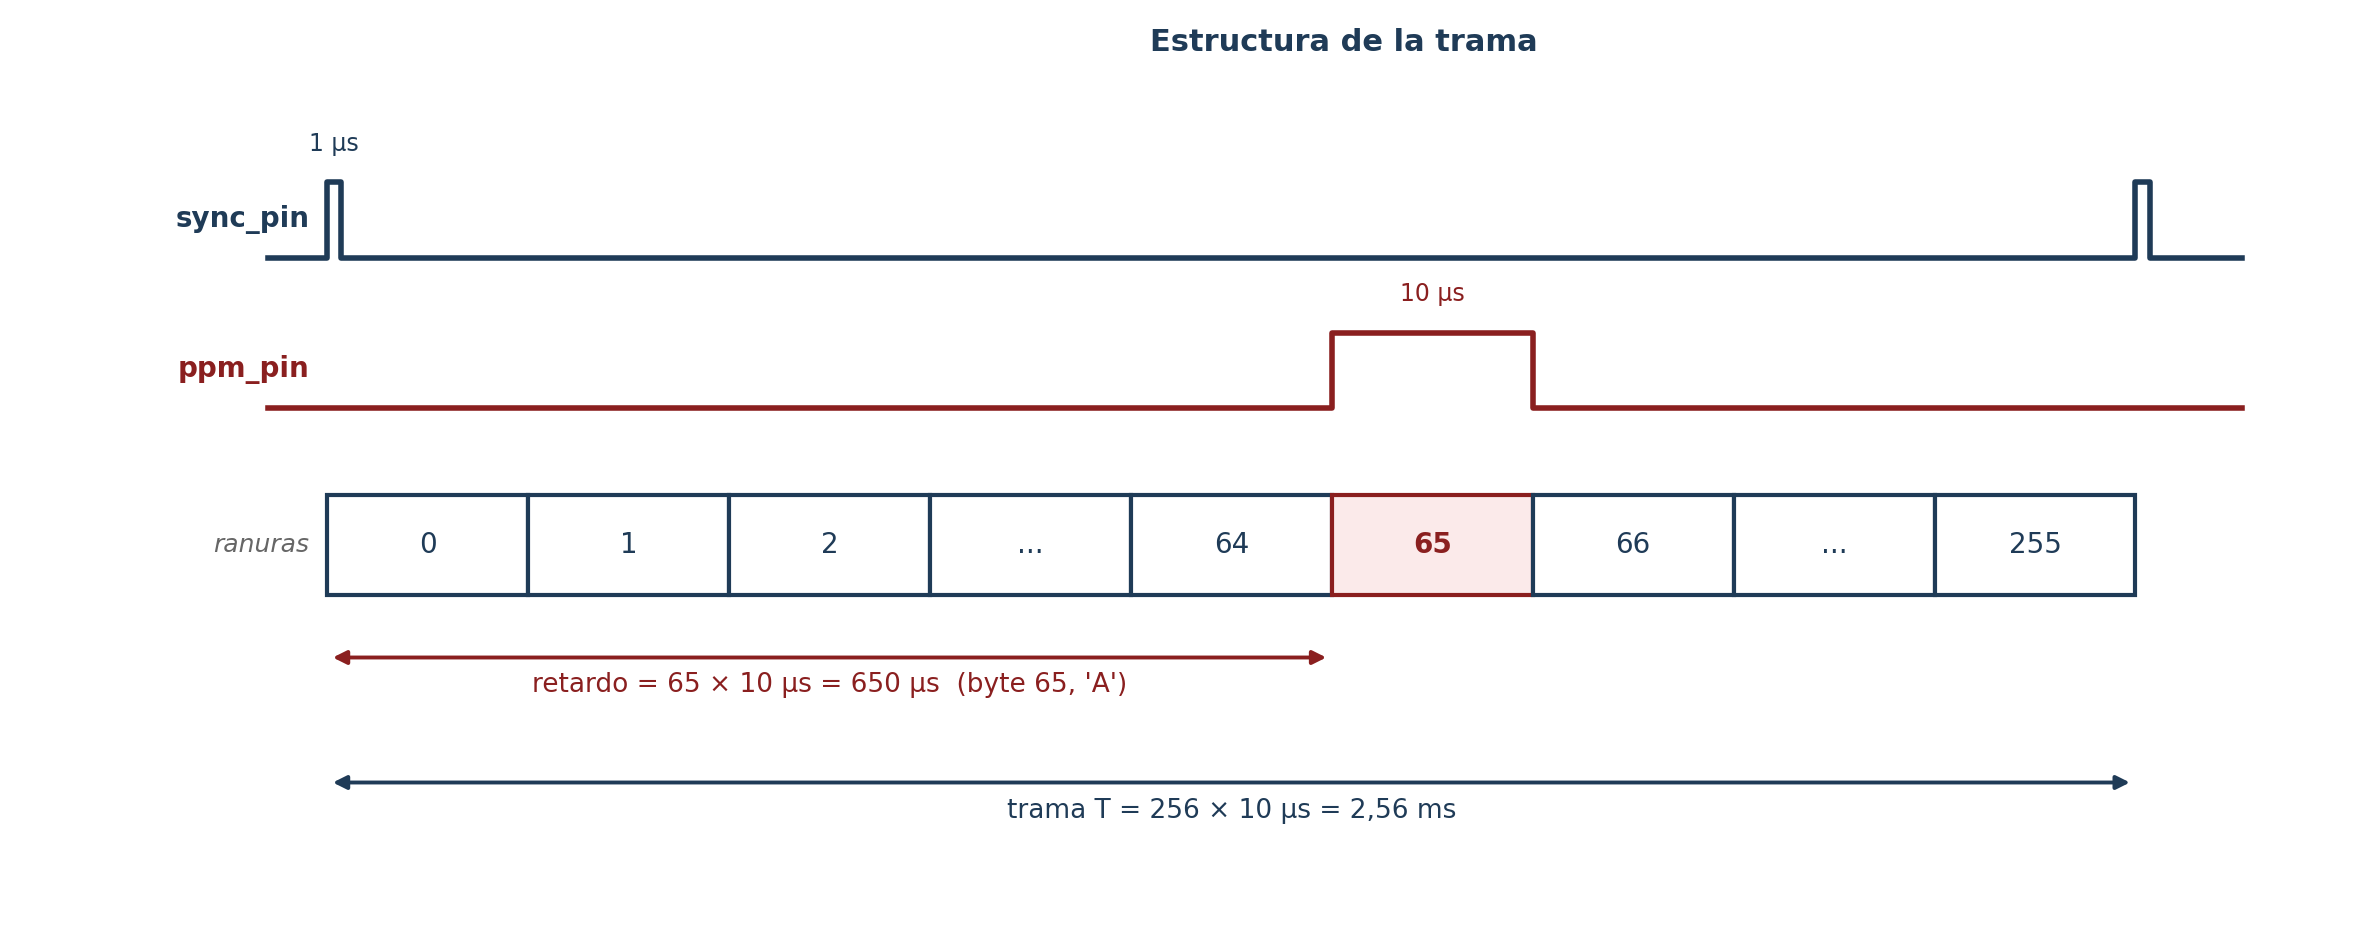
\includegraphics[width=\linewidth]{fig/trama.png}
  \caption{Estructura de la trama. \code{sync_pin} marca el comienzo; \code{ppm_pin} vale 1 durante la ranura cuyo número es el valor del byte.}
  \label{fig:trama}
\end{figure}



% =============================== 4. ARQUITECTURA ===============================
\section{Arquitectura}

\subsection{Diagrama en bloques}

El diseño se organiza en tres niveles: \code{uart_top} conecta los pines de la placa y fija los parámetros del
UART; \code{uart_ppm} une el receptor serie con el modulador y sincroniza el reset; \code{mod_ppm} convierte el
byte recibido en el pulso PPM.


\begin{figure}[H]
  \centering
  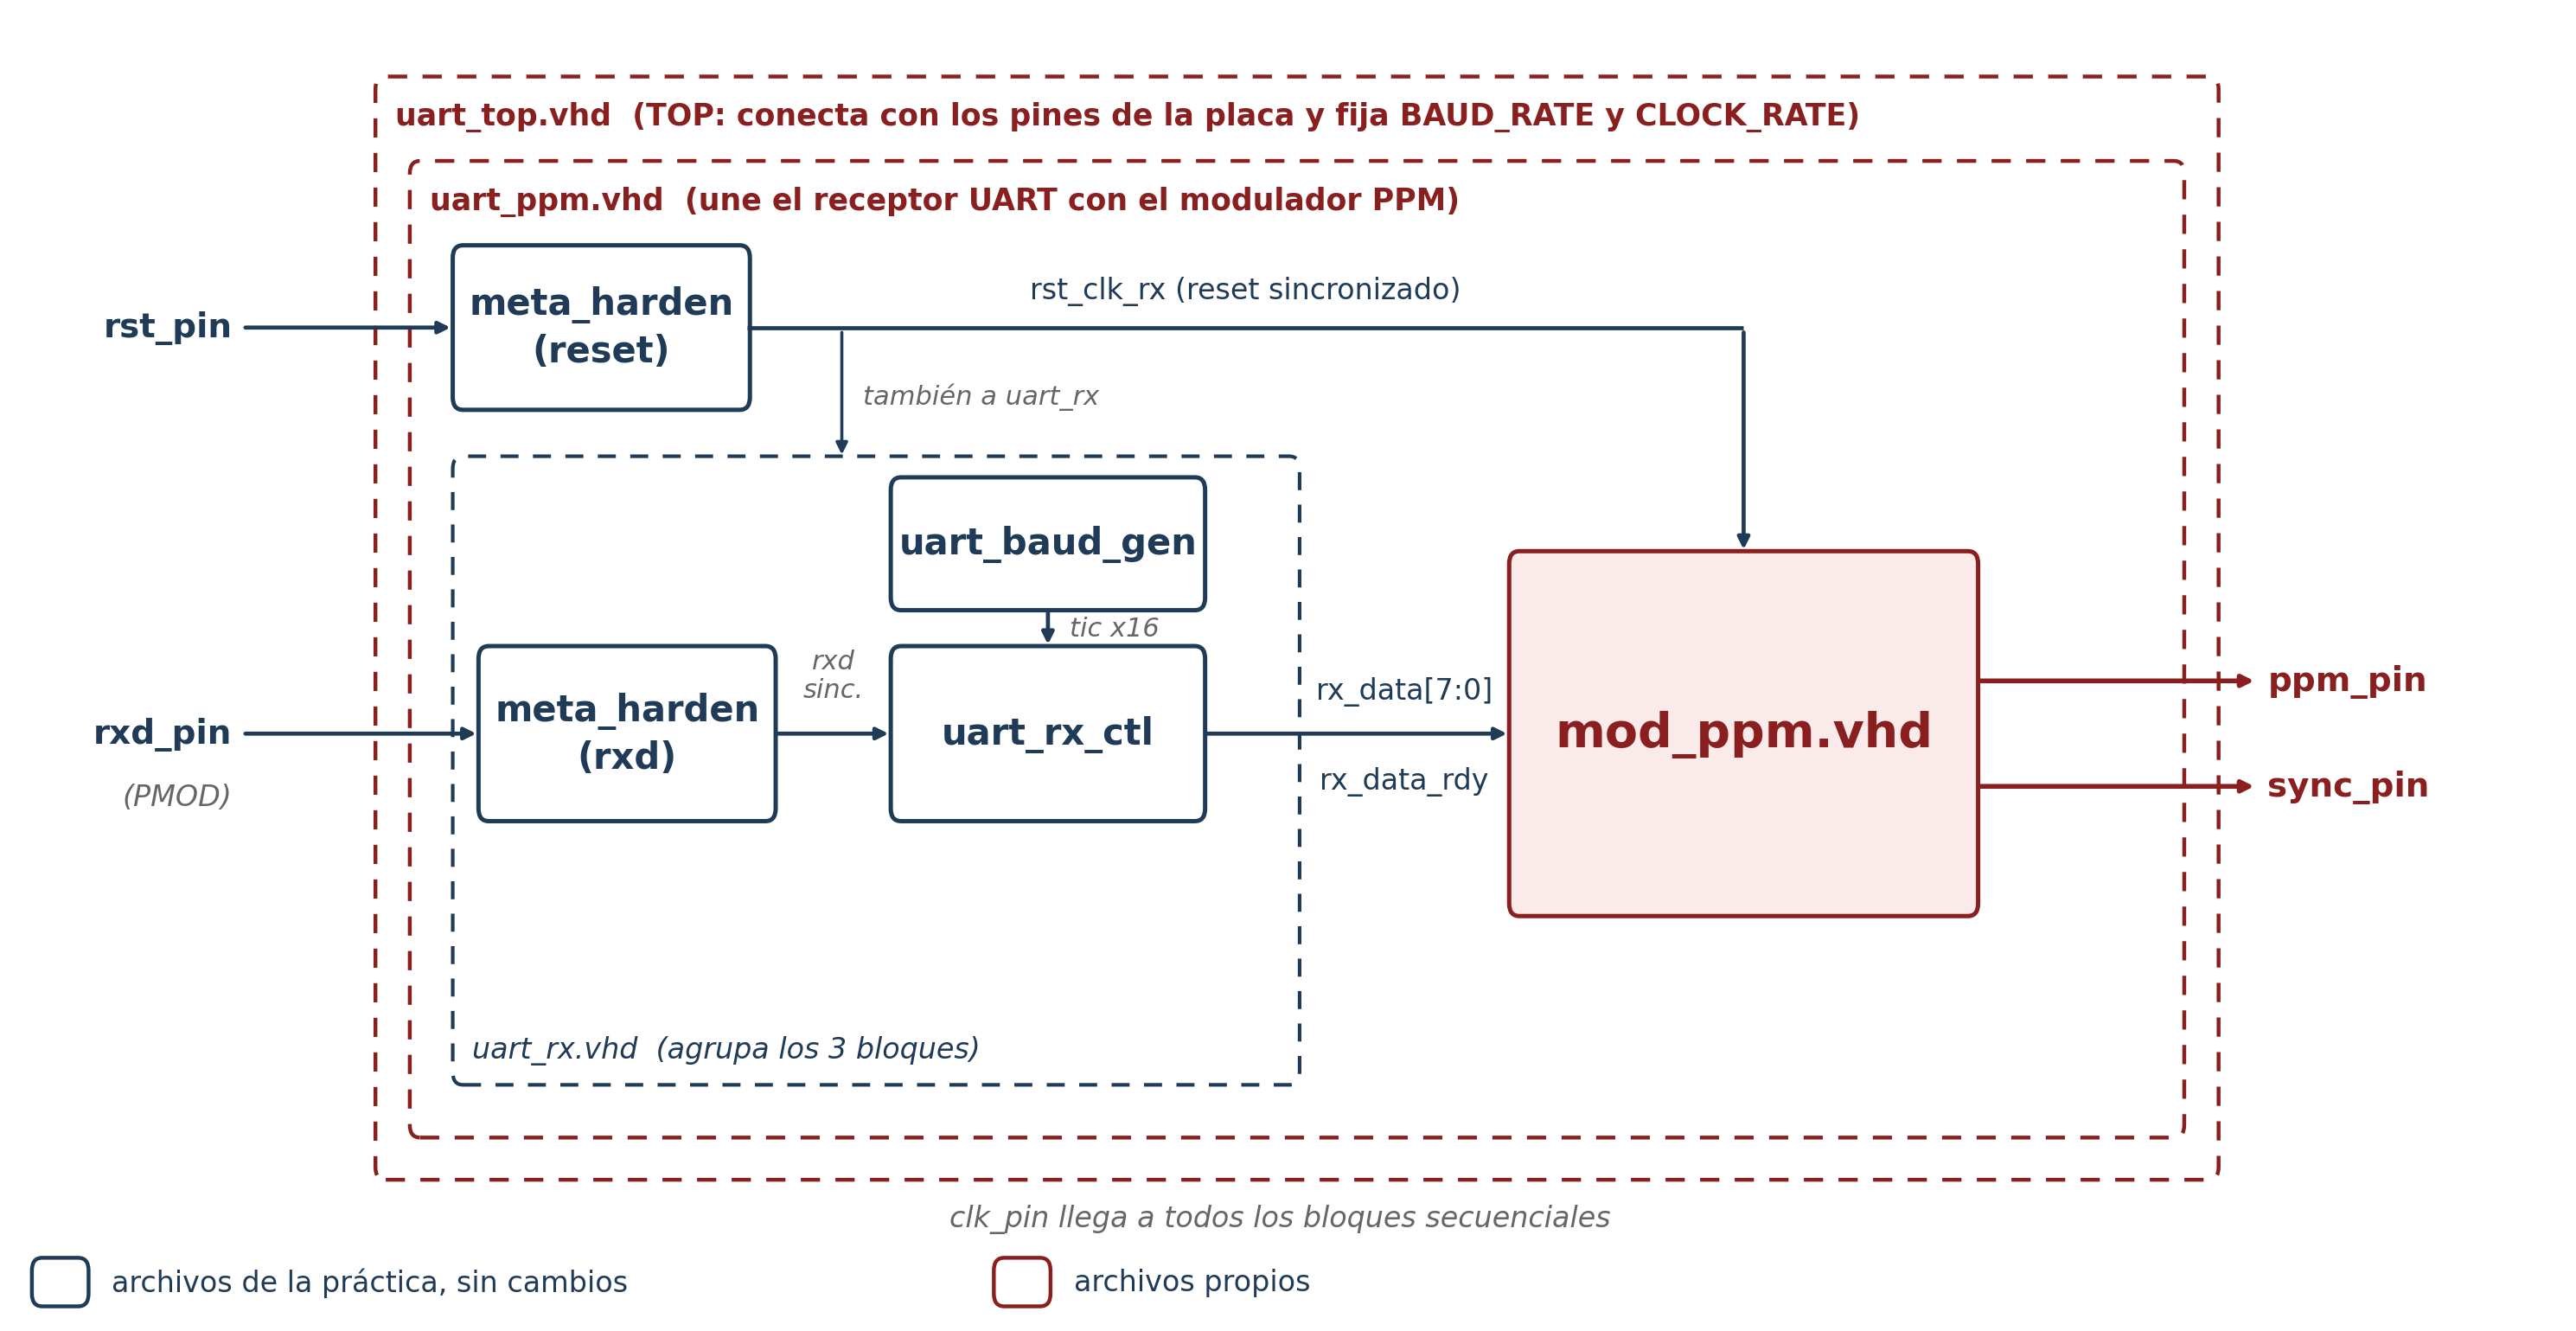
\includegraphics[width=0.75\linewidth]{fig/diagrama_bloques.png}
  \caption{Diagrama en bloques y archivos que contiene cada nivel. En azul, los archivos de la Práctica~2 sin cambios; en rojo, los propios.}
  \label{fig:bloques}
\end{figure}


\subsection{Archivos y bloques}

Los bloques del receptor UART y el sincronizador provienen de la Práctica~2 de la materia y se usan sin modificaciones. \code{uart_top} y \code{uart_ppm} siguen la estructura de \code{uart_top} y \code{uart_led} de esa práctica; \code{mod_ppm} es de elaboración propia y reemplaza al bloque que mostraba el
byte en los LEDs.

\begin{table}[H]
\centering
\small
\renewcommand{\arraystretch}{0.9}
\caption{Archivos VHDL del diseño.}
\label{tab:archivos}
\begin{tabularx}{\linewidth}{@{}l X l@{}}
\toprule
\textbf{Archivo} & \textbf{Función} & \textbf{Origen} \\
\midrule
\code{uart_top.vhd}      & Puertos externos y parámetros \code{BAUD_RATE} y \code{CLOCK_RATE} & Propio \\
\code{uart_ppm.vhd}      & Une el UART con el modulador; sincroniza el reset & Propio \\
\code{mod_ppm.vhd}       & Modulador PPM & Propio \\
\code{uart_rx.vhd}       & Receptor UART: agrupa sincronizador, generador de tics y control & Práctica 2 \\
\code{uart_rx_ctl.vhd}   & Máquina de estados de la recepción serie & Práctica 2 \\
\code{uart_baud_gen.vhd} & Generador de tics a 16 veces el baud rate & Práctica 2 \\
\code{meta_harden.vhd}   & Sincronizador de dos flip-flops para entradas asíncronas & Práctica 2 \\
\bottomrule
\end{tabularx}
\end{table}


\subsection{El módulo \texttt{mod\_ppm}}

\code{mod_ppm} tiene tres procesos sincrónicos, todos con reset sincrónico activo en alto:

\begin{itemize}
  \item \textbf{Contadores.} Dos contadores en cascada: uno cuenta los ciclos dentro de la ranura (de 0 a 1249) y otro las ranuras dentro de la trama (de 0 a 255). El segundo avanza cuando el primero completa su vuelta; cuando ambos llegan a su máximo comienza una trama nueva.
  \item \textbf{Byte.} Captura el byte en el flanco de subida de \code{rx_data_rdy_i} y levanta el flag \code{byte_waiting}. Al comienzo de cada trama, si hay un byte esperando lo pasa al registro de comparación, baja el flag y marca la trama como con mensaje; si no hay, la marca como vacía. Para esto usa el flag \code{empty_msg}.
  \item \textbf{Salidas.} \code{ppm_o} vale 1 cuando la trama tiene mensaje y la ranura actual es igual al byte; \code{sync_o} vale 1 durante los primeros 125 ciclos de la trama.
\end{itemize}

\begin{table}[H]
\centering
\small
\renewcommand{\arraystretch}{0.9}
\caption{Parámetros y señales internas de \code{mod_ppm}.}
\label{tab:senales}
\begin{tabularx}{\linewidth}{@{}l X@{}}
\toprule
\textbf{Señal / generic} & \textbf{Función} \\
\midrule
\code{CYCLES_PER_SLOT} = 1250 & Ciclos de clock por ranura (\SI{10}{\micro\second} a \SI{125}{\mega\hertz}) \\
\code{NUM_SLOTS} = 256 & Ranuras por trama \\
\code{W_SYNC} = 125 & Ciclos que dura \code{sync_o} en alto (\SI{1}{\micro\second}) \\
\code{cycle_count}, \code{window_count} & Contadores de ciclos y de ranuras \\
\code{old_rx_data_rdy} & Valor anterior de \code{rdy}, para detectar su flanco de subida \\
\code{arrival_byte} & Último byte capturado \\
\code{byte_waiting} & Hay un byte capturado que todavía no se usó \\
\code{compare_byte} & Byte que se compara con el contador de ranuras en la trama actual \\
\code{empty_msg} & 1: la trama va vacía; 0: la trama lleva un pulso \\
\bottomrule
\end{tabularx}
\end{table}

% =============================== 5. SIMULACION ===============================
\section{Simulaciones}

\subsection{Entorno}

Las simulaciones se realizaron con ModelSim Intel FPGA Edition 2020.1. Los testbenches de \code{mod_ppm} usan
\emph{generics} reducidos (4 ciclos por ranura y pocas ranuras) para que una trama completa se vea en pocas
decenas de ciclos, con el mismo comportamiento que con los valores reales. El testbench del sistema completo
usa los valores reales de \SI{125}{\mega\hertz} y \num{115200} baudios.

\subsection{Testbenches}

Se desarrollaron cinco testbenches (tabla~\ref{tab:tbs}). Los cuatro primeros prueban \code{mod_ppm} de forma
aislada, inyectando directamente el byte y la señal \code{rdy} que entregaría el receptor UART, y cada uno se
enfoca en un comportamiento del módulo: la posición del pulso para un byte, el desplazamiento del pulso entre
tramas consecutivas, la regla de que gana el primer byte cuando llegan varios en la misma trama, y la captura
de un único byte aunque \code{rdy} permanezca en alto durante varias tramas. El último testbench prueba el
sistema completo: envía tres bytes por la línea serie a \num{115200} baudios y comprueba toda la cadena, desde el
receptor UART hasta el pulso de salida. En todos los casos el resultado fue el esperado.

\begin{table}[H]
\centering
\caption{Testbenches y resultados.}
\label{tab:tbs}
\small
\begin{tabularx}{\linewidth}{@{}l X X@{}}
\toprule
\textbf{Testbench} & \textbf{Qué verifica} & \textbf{Resultado} \\
\midrule
\code{mod_ppm_tb1_basico} & Un byte (de valor 10) llega durante la primera trama; trama de 12 ranuras. & Pulso en la ranura 10 de la trama siguiente. \\
\code{mod_ppm_tb2_secuencia} & Bytes 0, 1, 2 y 3, uno por trama (4 ranuras). & Un pulso por trama, en las ranuras 0, 1, 2 y 3. \\
\code{mod_ppm_tb3_primero} & Dos bytes (5 y 2) en la misma trama. & Un solo pulso, en la ranura 5; el 2 se descarta. \\
\code{mod_ppm_tb4_rdylargo} & \code{rdy} en alto durante varias tramas con el byte 3. & Un solo pulso; las tramas siguientes van vacías. \\
\code{uart_top_tb} & Sistema completo: los bytes 5, 65 y 122 se envían por la línea serie, uno por trama. & Un pulso por byte, en la trama siguiente a su llegada, en las ranuras 5, 65 y 122. \\
\bottomrule
\end{tabularx}
\end{table}

\newpage
\subsubsection{Testbench 1: \texttt{mod\_ppm\_tb1\_basico}}

Este testbench env\'ia un \'unico byte de valor 10 a un \code{mod_ppm} con 12 ranuras de 4 ciclos de reloj, con un per\'iodo de \SI{100}{\nano\second} (\SI{10}{\mega\hertz}). Con estos par\'ametros reducidos el pulso de sincronismo dura \SI{200}{\nano\second} (2 ciclos), el pulso de dato ocupa una ranura de \SI{400}{\nano\second} (4 ciclos) y la trama completa dura \SI{4800}{\nano\second}. En la figura~\ref{fig:simtb1} se ve que el pulso de \code{rdy} que entrega el byte ocurre durante la primera trama, que va vac\'ia, y que el pulso de \code{ppm} aparece reci\'en en la trama siguiente.

\begin{figure}[H]
  \centering
  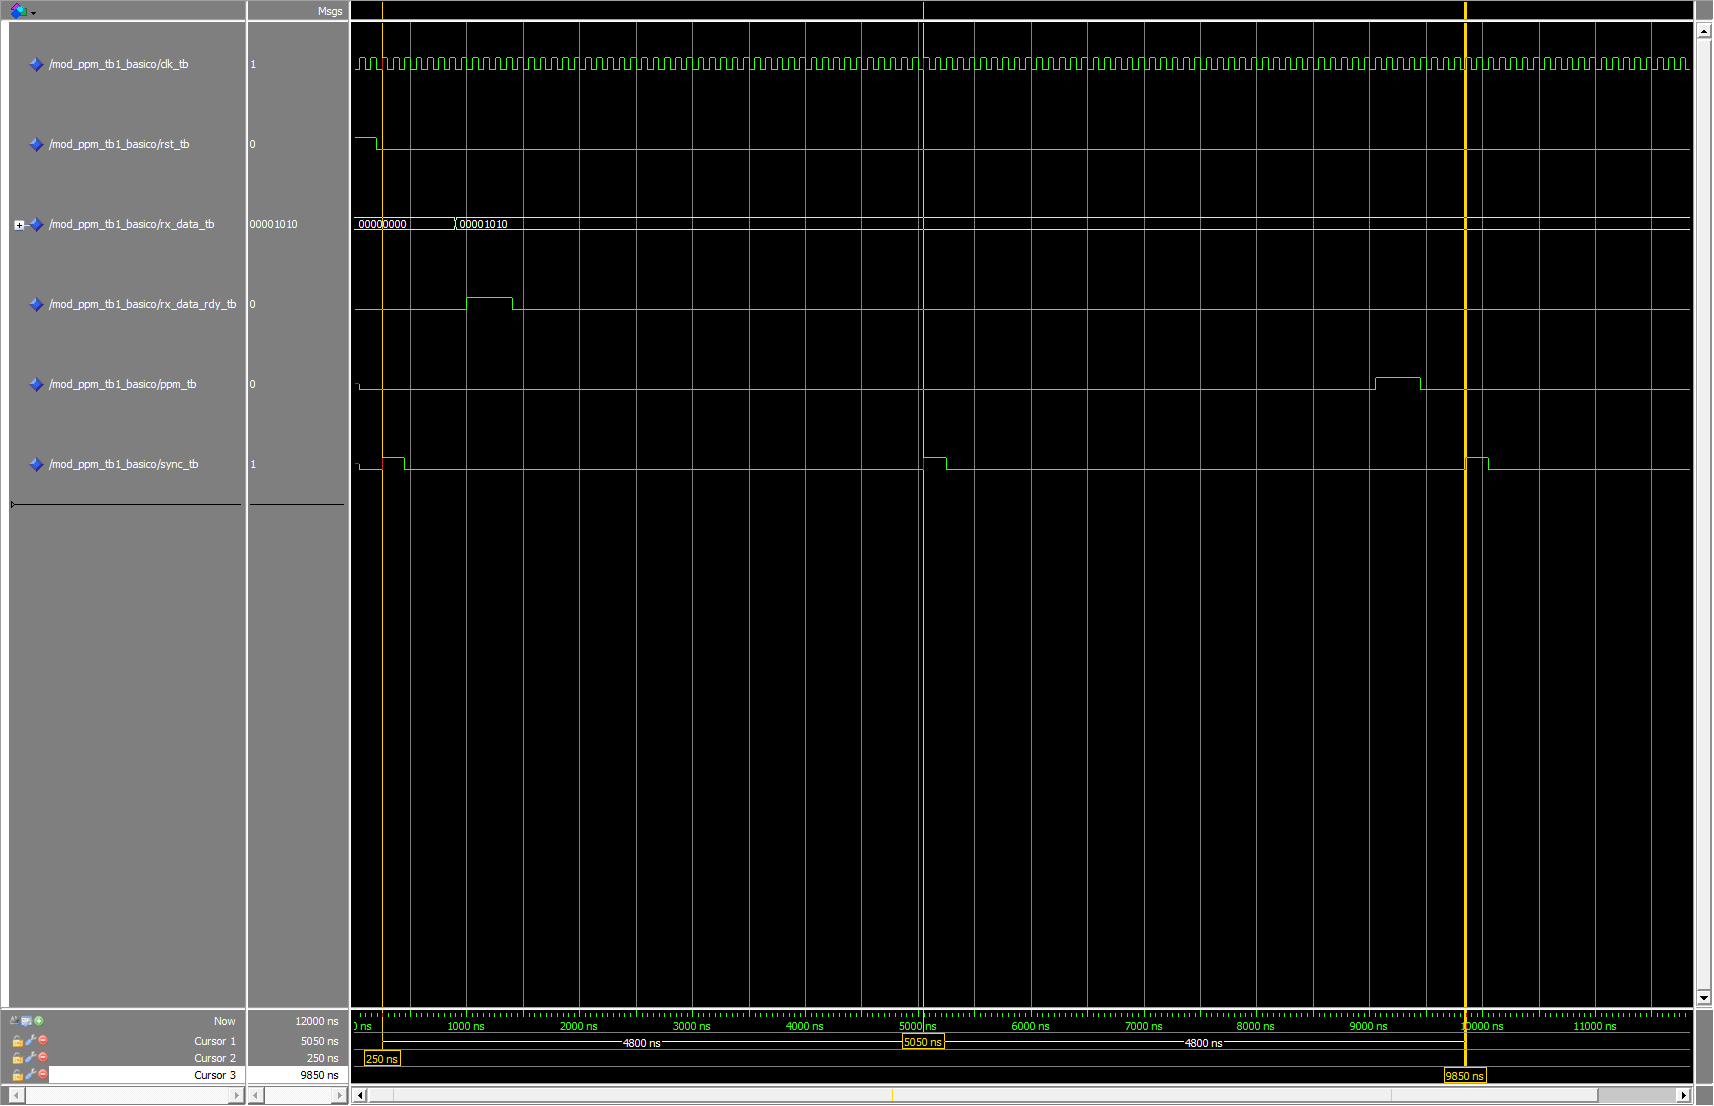
\includegraphics[width=0.95\linewidth]{fig/sim_tb1.png}
  \caption{Simulación de \code{mod_ppm_tb1_basico}: el byte 10 llega durante la primera trama y el pulso aparece en la ranura 10 de la trama siguiente.}
  \label{fig:simtb1}
\end{figure}

\newpage

\subsubsection{Testbench 2: \texttt{mod\_ppm\_tb2\_secuencia}}

Se envían los bytes 0, 1, 2 y 3, uno por trama, a un módulo de 4 ranuras de 4 ciclos (tramas de
\SI{1600}{\nano\second}, que los cursores de la figura~\ref{fig:simtb2} confirman entre un \code{sync} y el
siguiente). Cada byte, acompañado por su pulso de \code{rdy}, se usa en la trama que sigue, y el pulso de
\code{ppm} se corre una ranura hacia la derecha en cada trama: sale en la ranura 0, 1, 2 y 3. El primero coincide
con el flanco del \code{sync}, porque el byte 0 ocupa la primera ranura. Esta es la simulación que mejor muestra
la modulación, con el pulso moviéndose según el dato.

\begin{figure}[H]
  \centering
  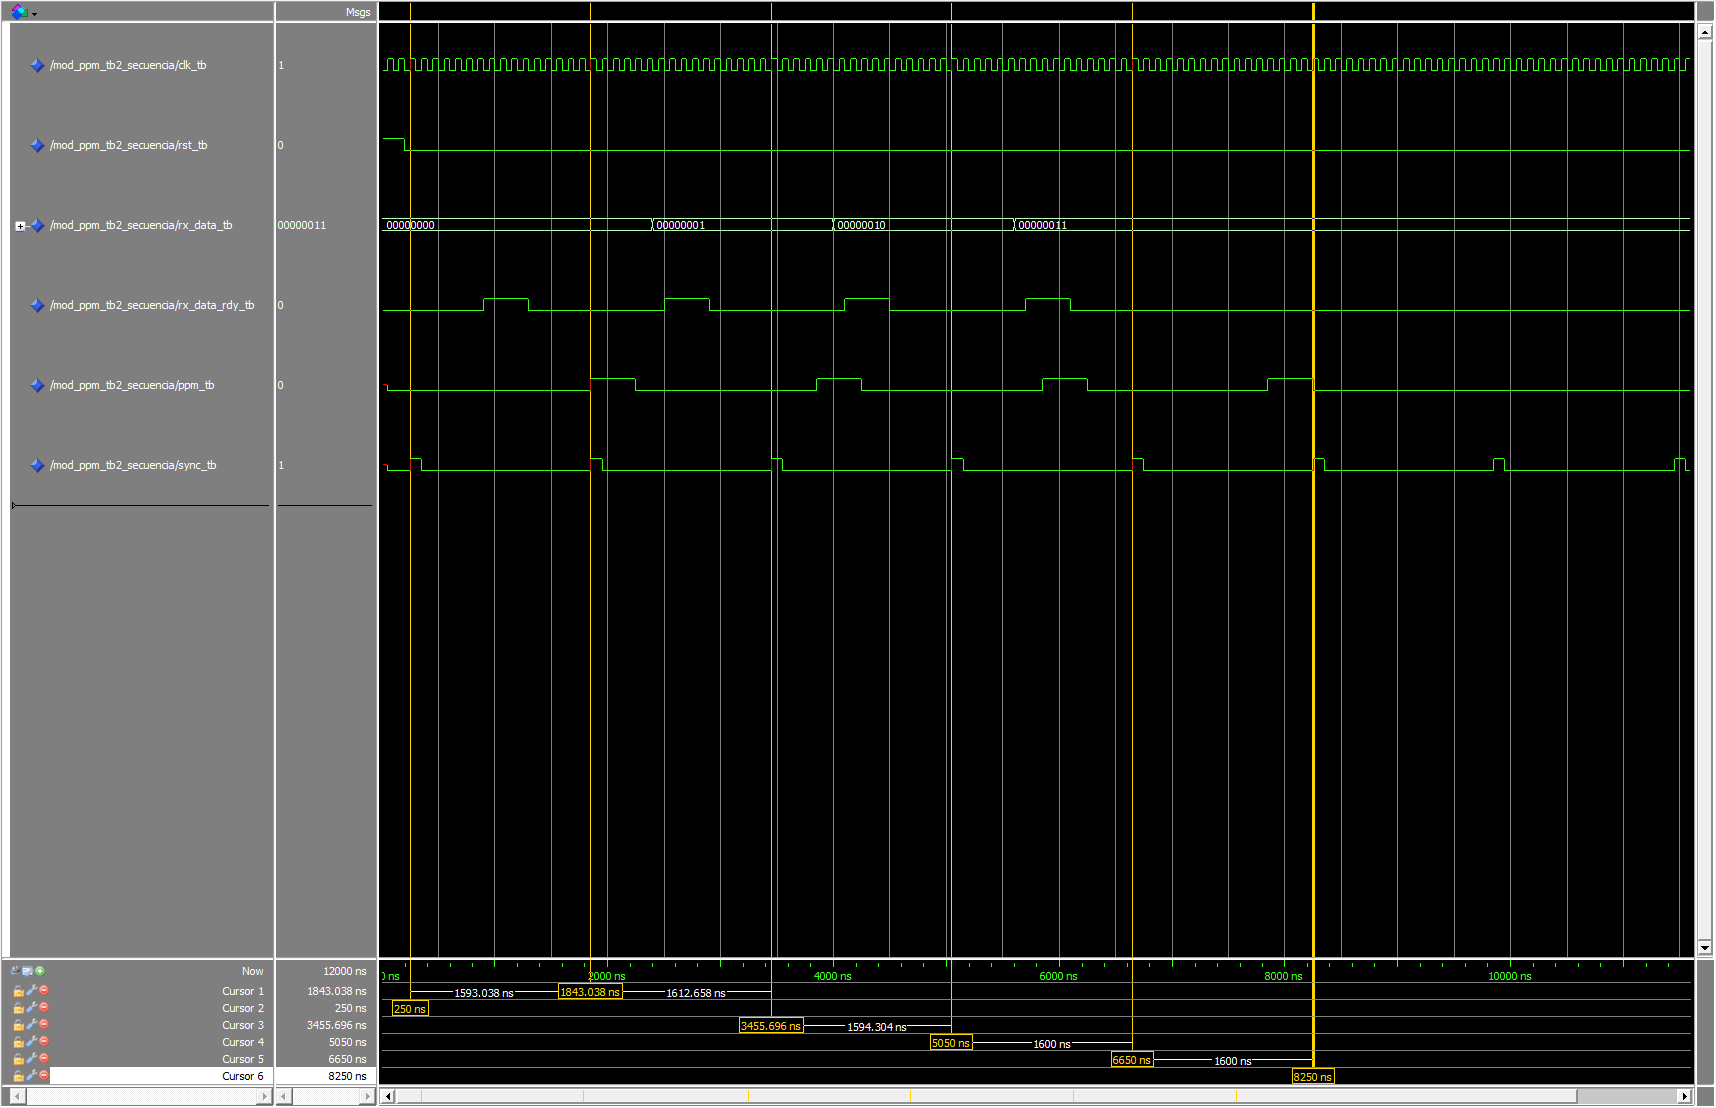
\includegraphics[width=0.95\linewidth]{fig/sim_tb2.png}
  \caption{Simulación de \code{mod_ppm_tb2_secuencia}: con los bytes 0, 1, 2 y 3, el pulso de \code{ppm} se desplaza una ranura en cada trama.}
  \label{fig:simtb2}
\end{figure}

\newpage

\subsubsection{Testbench 3: \texttt{mod\_ppm\_tb3\_primero}}

Este testbench verifica la regla de que gana el primer byte. Durante la primera trama llegan dos bytes seguidos,
el 5 (\code{00000101}) y el 2 (\code{00000010}), cada uno con su pulso de \code{rdy} (figura~\ref{fig:simtb3}).
En la trama siguiente, que empieza en \SI{3450}{\nano\second}, aparece un único pulso de \code{ppm}, en la ranura
5. No hay ningún pulso en la ranura 2 ni en las tramas posteriores, de modo que el segundo byte se descartó, y
cada trama dura \SI{3200}{\nano\second}, como indican los cursores sobre los \code{sync}.

\begin{figure}[H]
  \centering
  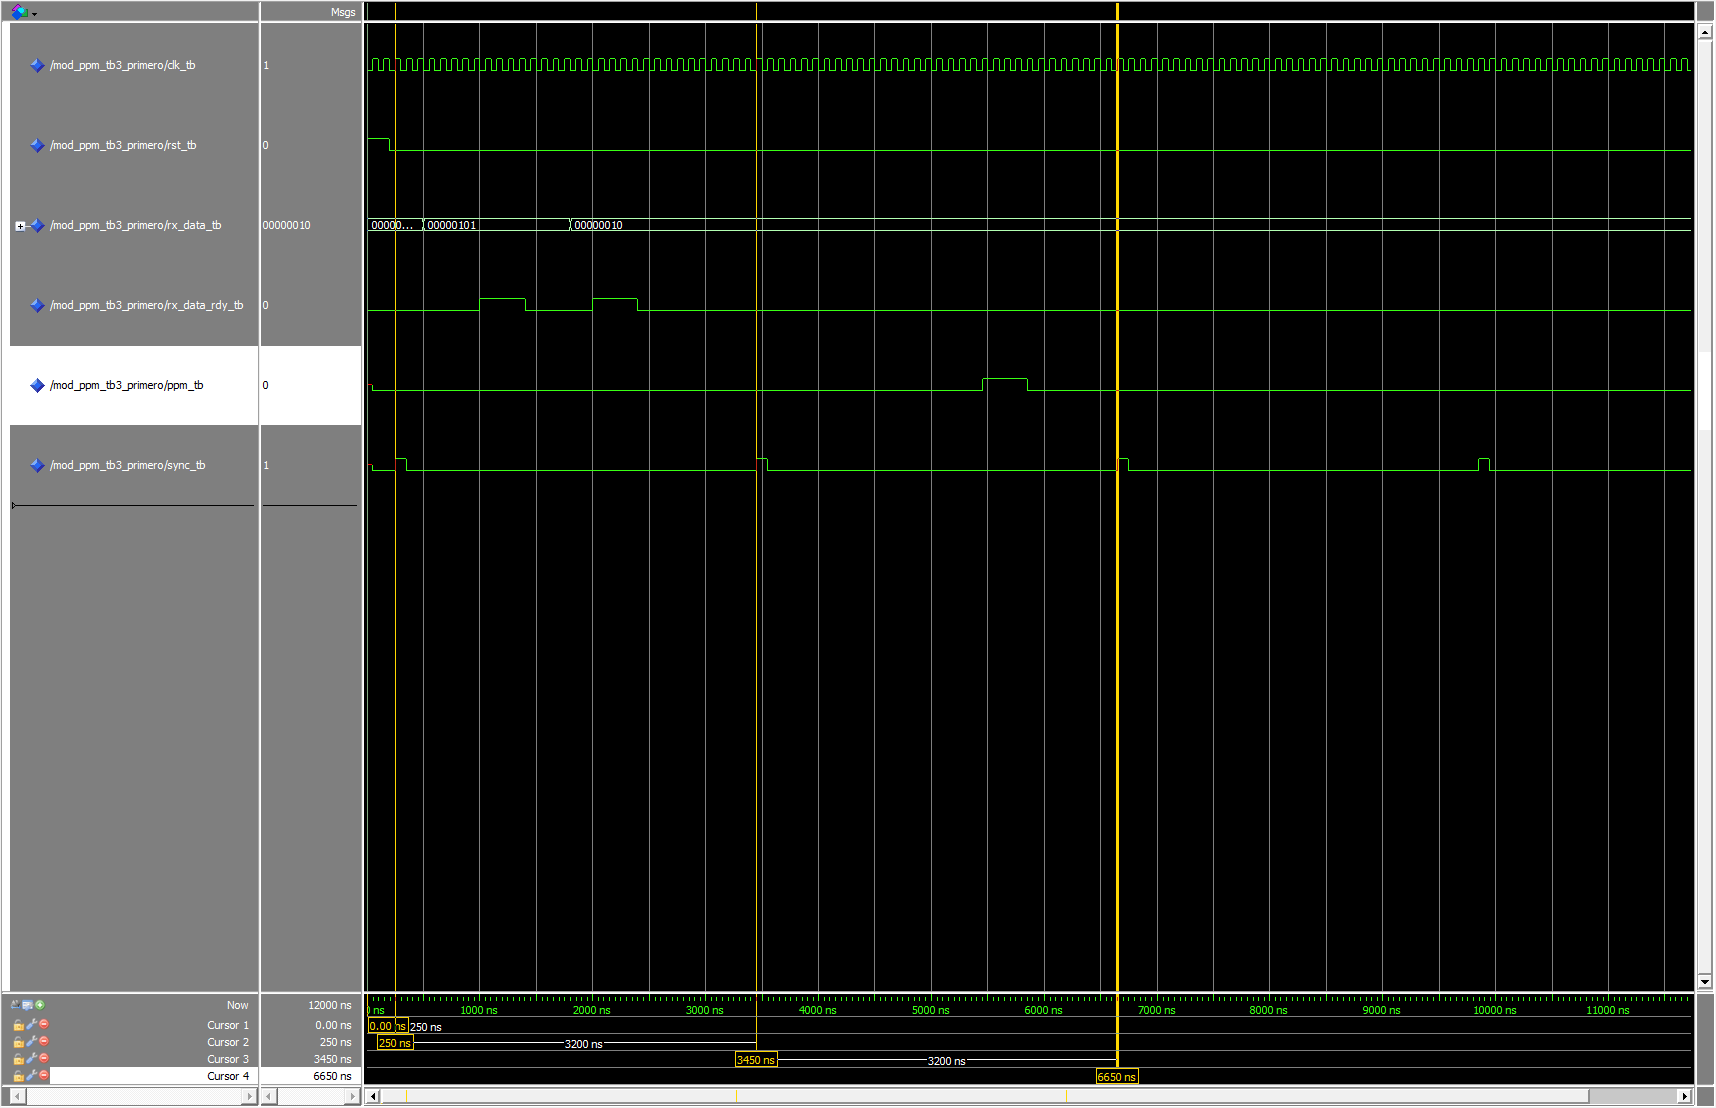
\includegraphics[width=0.95\linewidth]{fig/sim_tb3.png}
  \caption{Simulación de \code{mod_ppm_tb3_primero}: con los bytes 5 y 2 en la misma trama, solo se modula el primero.}
  \label{fig:simtb3}
\end{figure}

\newpage
\subsubsection{Testbench 4: \texttt{mod\_ppm\_tb4\_rdylargo}}

En este caso el byte 3 llega con \code{rdy} en alto durante \SI{8,7}{\micro\second},y en este testbench abarca casi tres tramas (figura~\ref{fig:simtb4}). A pesar de eso, \code{ppm} produce un
único pulso, en la ranura 3 de la segunda trama, y la tercera trama va vacía aunque \code{rdy} siga en alto
durante buena parte de ella. Esto muestra que el byte se captura solo en el flanco de subida de \code{rdy}, y no
mientras la señal permanece activa, lo que evita repetir el mismo pulso en las tramas siguientes.

\begin{figure}[H]
  \centering
  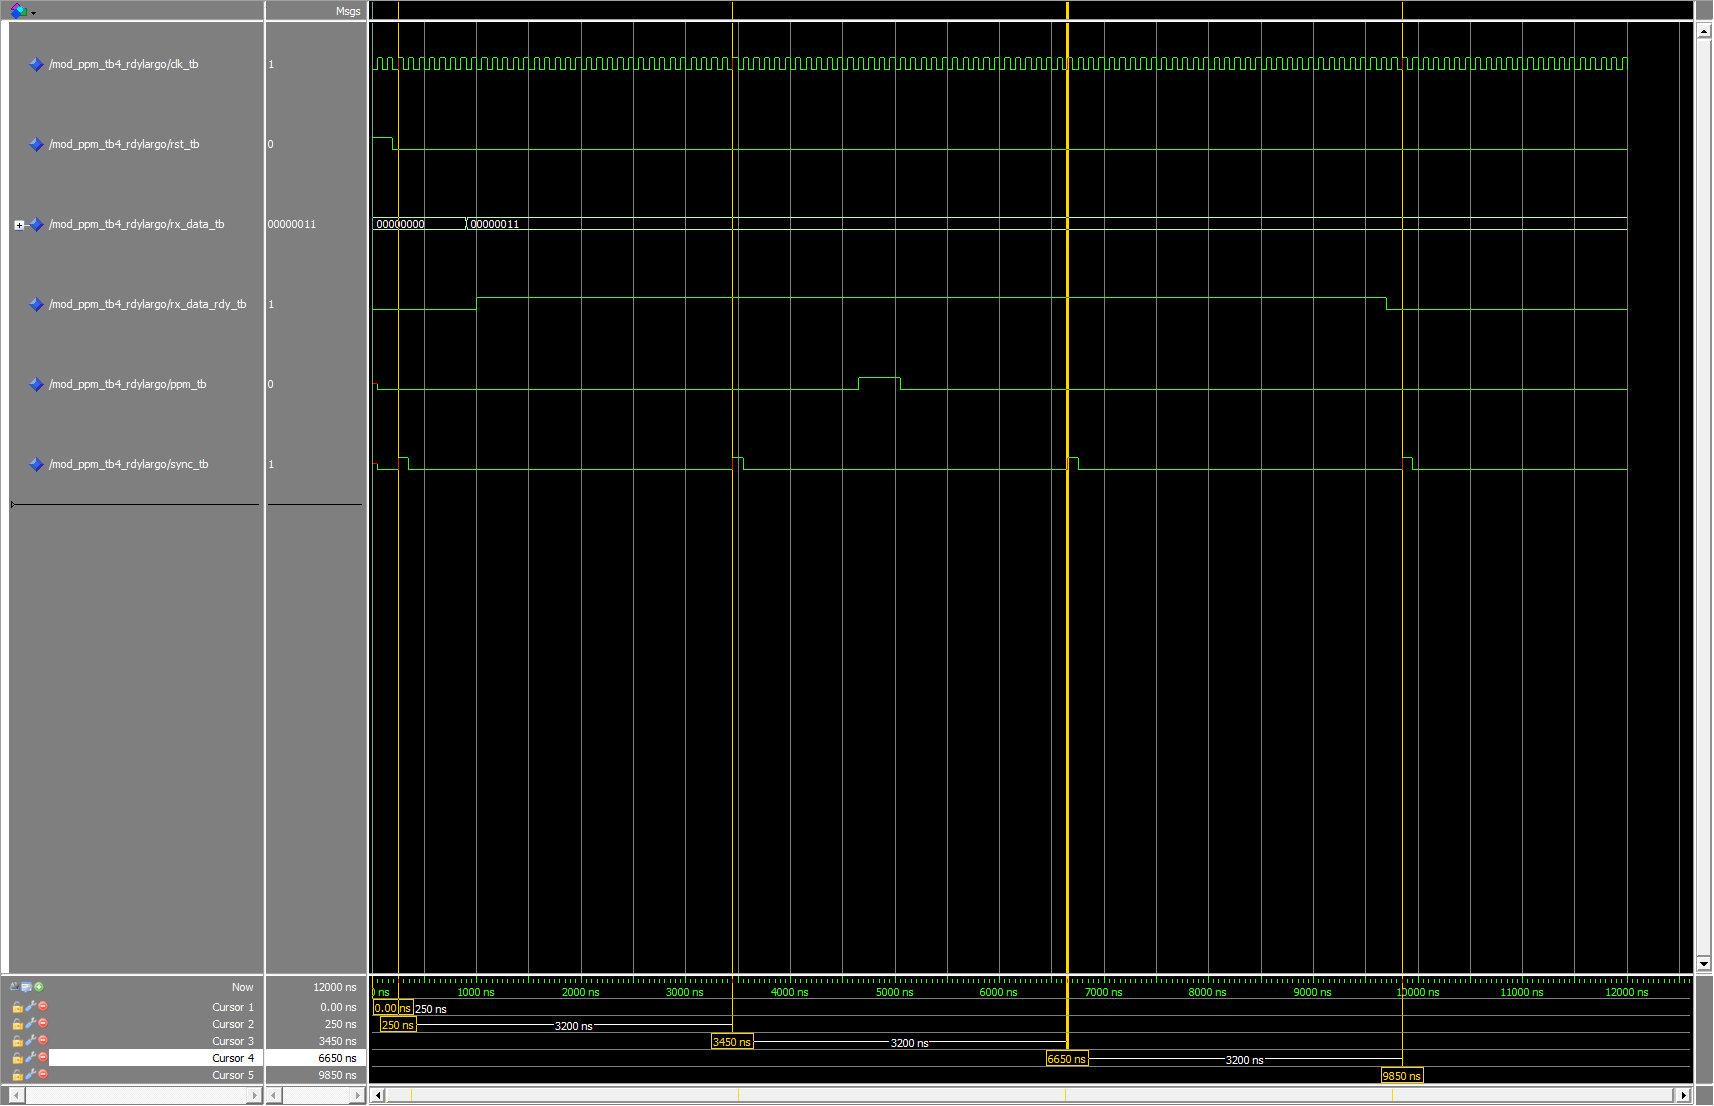
\includegraphics[width=0.95\linewidth]{fig/sim_tb4.png}
  \caption{Simulación de \code{mod_ppm_tb4_rdylargo}: con \code{rdy} en alto durante varias tramas, el byte genera un solo pulso.}
  \label{fig:simtb4}
\end{figure}

\newpage
\subsubsection{Testbench 5: \texttt{uart\_top\_tb}}

Este testbench prueba el sistema completo con los valores reales: un clock de \SI{125}{\mega\hertz} y una línea
serie de \num{115200} baudios, por la que se envían tres bytes sucesivos, cada uno con su bit de start, los
8 bits de datos (primero el menos significativo) y el bit de stop. Los bytes son el 5, el 65 (\texttt{'A'}) y el
122 (\texttt{'z'}), enviados a partir de los \SI{100}{\micro\second}, \SI{3000}{\micro\second} y
\SI{6000}{\micro\second}, de modo que cada uno llega durante una trama distinta, cuando el anterior ya se está
modulando. Como los tres valores están bien separados, en la figura~\ref{fig:simtb5} se ve cómo el pulso se desplaza hacia la derecha de una trama a la siguiente.

\begin{figure}[H]
  \centering
  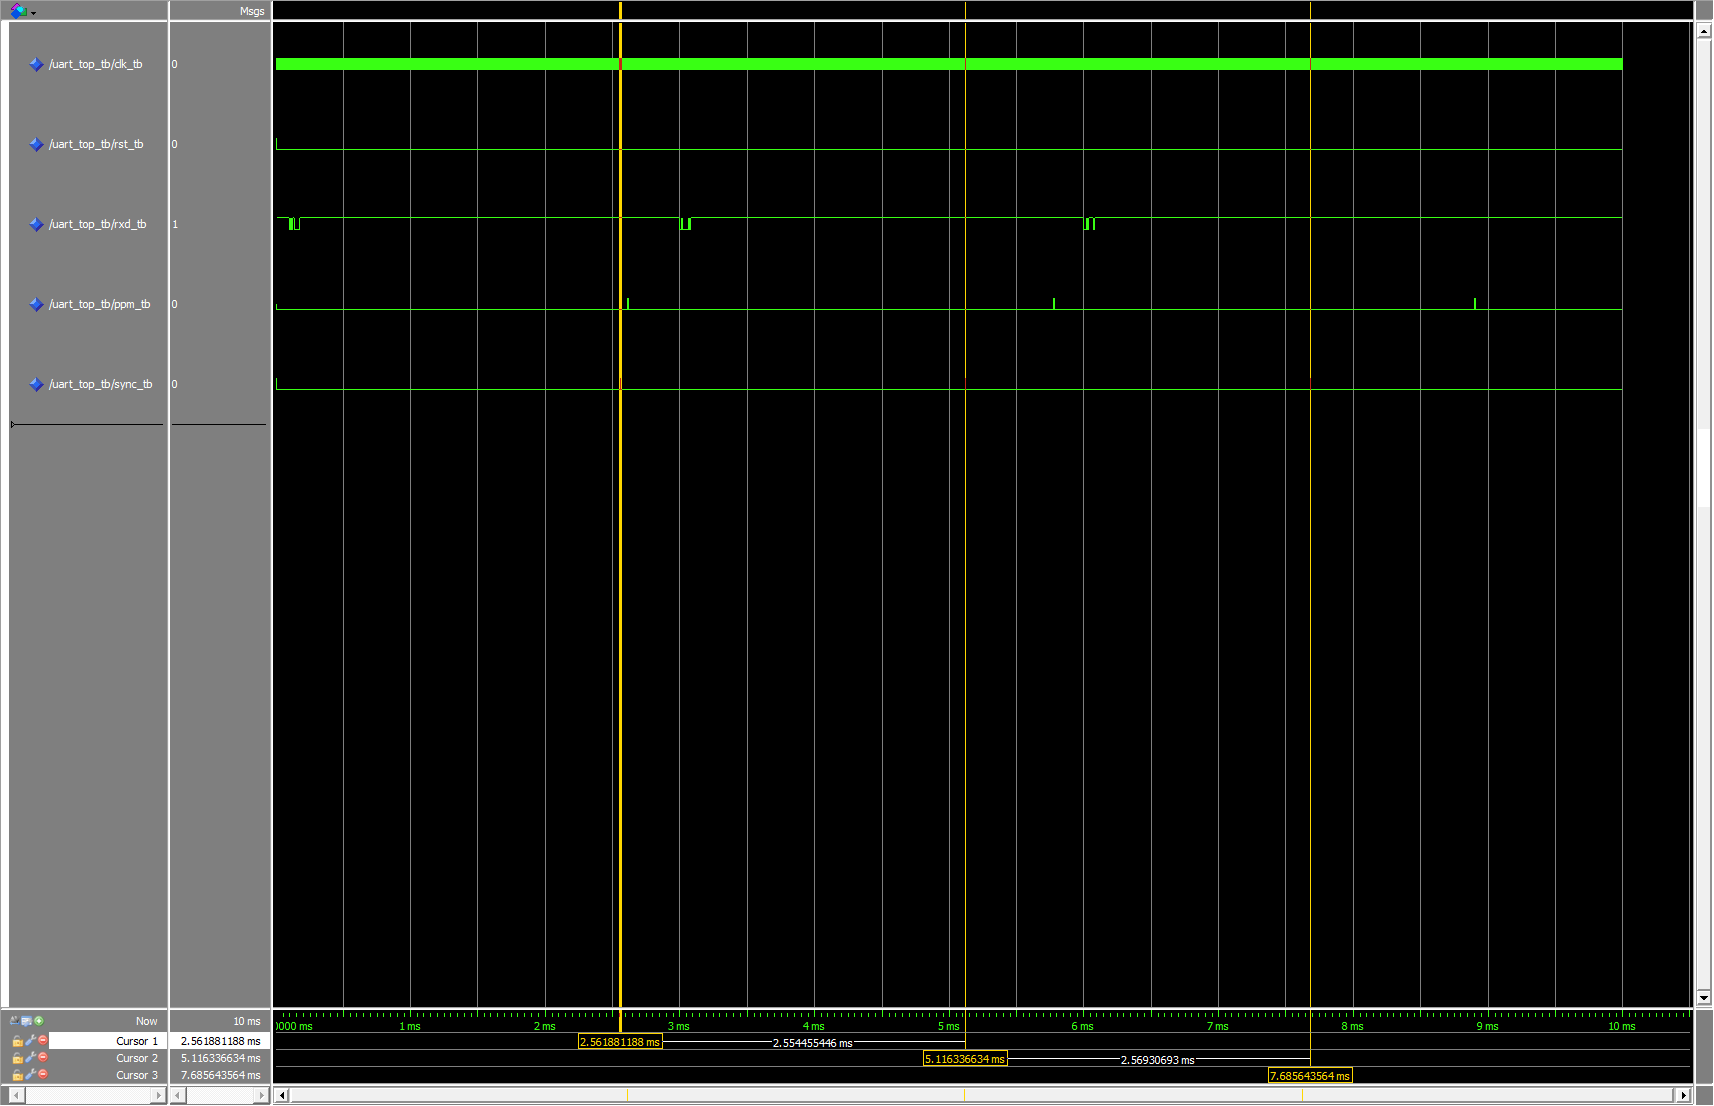
\includegraphics[width=0.95\linewidth]{fig/sim_tb5.png}
  \caption{Simulación del sistema completo (\code{uart_top_tb}) durante \SI{10}{\milli\second}: los tres bytes enviados por \code{rxd} producen tres pulsos de \code{ppm}, cada uno en la trama siguiente y más desplazado respecto del \code{sync} que la abre (marcado por los cursores, separados unos \SI{2,56}{\milli\second}). El clock se ve como una banda continua por la escala de tiempo.}
  \label{fig:simtb5}
\end{figure}

En la figura~\ref{fig:simtb52} se amplía la simulación alrededor del segundo flanco de sincronismo para medir los anchos de los pulsos. Se verifica que el pulso de sincronismo dura \SI{1}{\micro\second} y que el pulso de dato ocupa exactamente una ranura de \SI{10}{\micro\second}.

\begin{figure}[H]
  \centering
  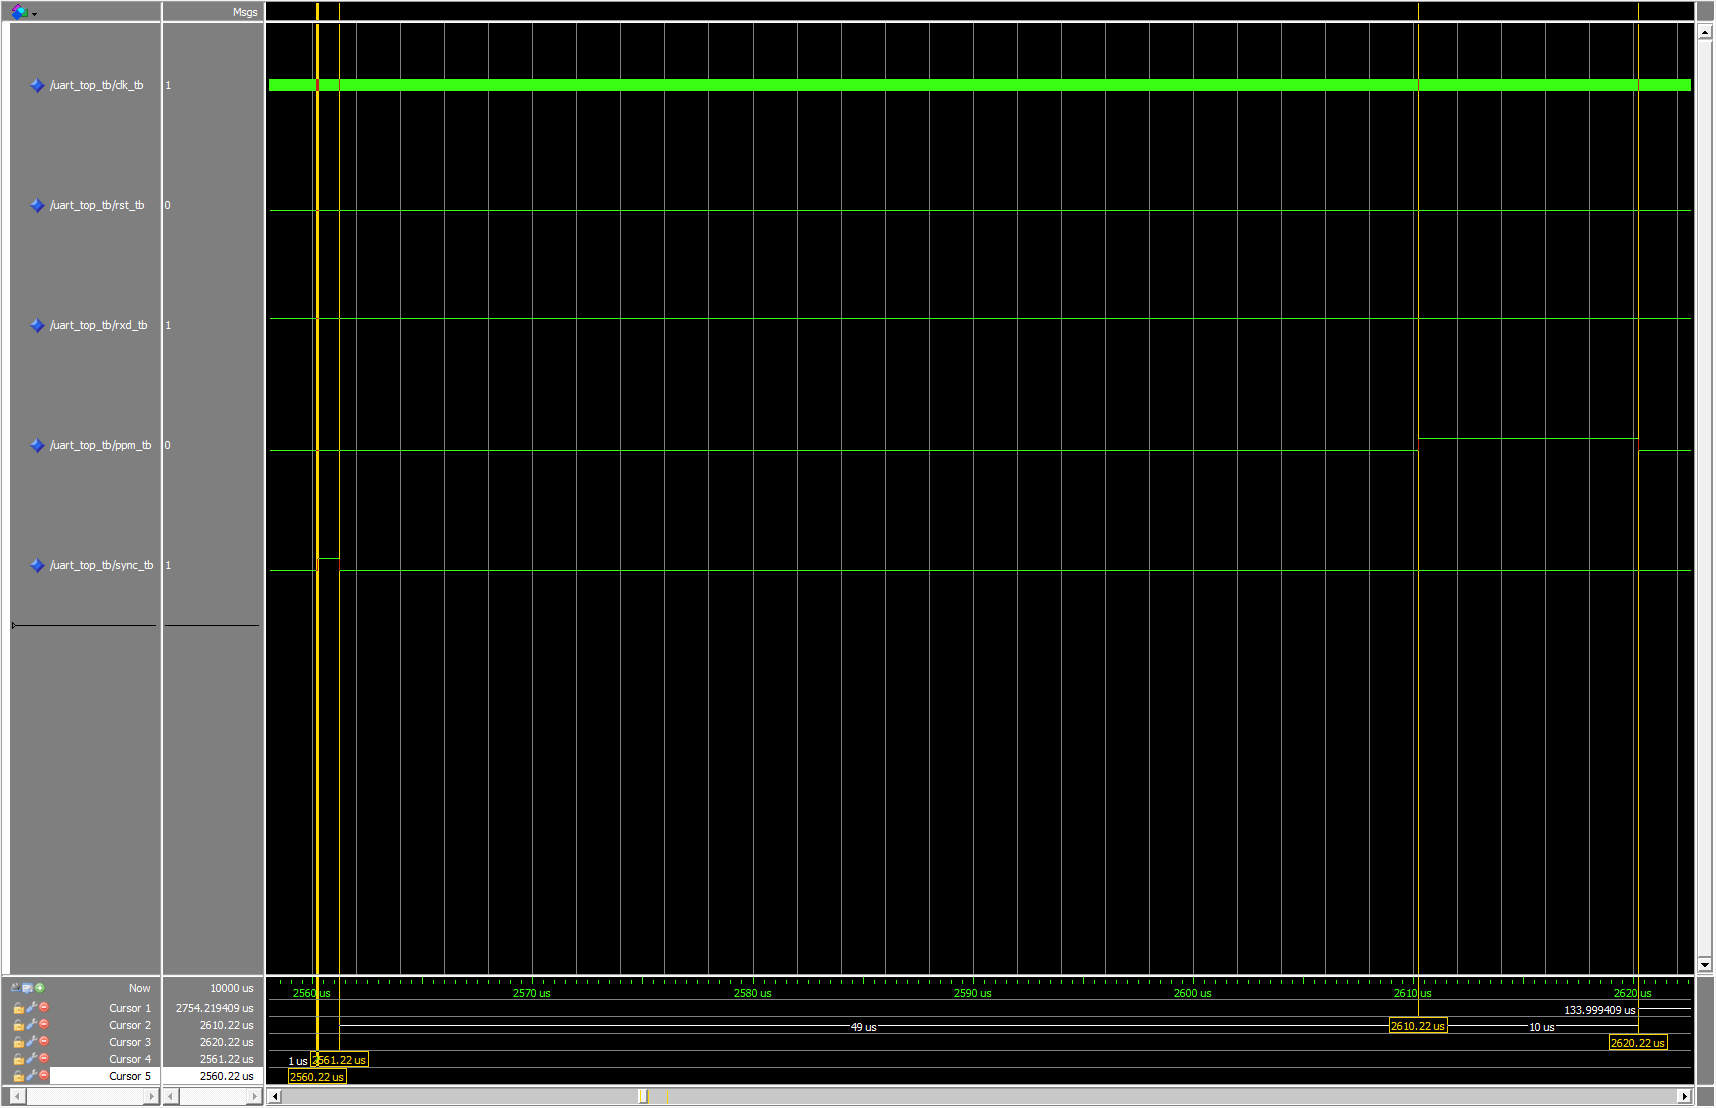
\includegraphics[width=0.95\linewidth]{fig/sim_tb5_2.png}
\caption{Simulaci\'on en ModelSim de los anchos de pulso: el pulso de sincronismo (\texttt{sync\_pin}) dura \SI{1}{\micro\second} (cursores en \SI{2560,22}{\micro\second} y \SI{2561,22}{\micro\second}) y el pulso de dato (\texttt{ppm\_pin}) dura \SI{10}{\micro\second}, una ranura (cursores en \SI{2610,22}{\micro\second} y \SI{2620,22}{\micro\second}).}
  \label{fig:simtb52}
\end{figure}



% =============================== 6. IMPLEMENTACION ===============================
\section{Síntesis e implementación}

\subsection{Archivos}

Se creó un proyecto de Vivado 2018.3 para la Arty Z7-10 con las siete fuentes VHDL y dos archivos .xdc:

\begin{itemize}
  \item \code{uart_ppm_pins_ArtyZ7.xdc} asigna cada puerto del top a su pin.
  \item \code{uart_ppm_timing_ArtyZ7.xdc} contiene la definición del clock de \SI{125}{\mega\hertz}.
\end{itemize}

\subsection{Esquemático}

El esquem\'atico generado por Vivado tras la elaboraci\'on del dise\~no se muestra en dos niveles. En la figura~\ref{fig:esqtop} se ve el nivel superior, donde \code{uart_ppm} aparece como una caja con las tres entradas (\code{clk_pin}, \code{rst_pin} y \code{rxd_pin}) y las dos salidas (\code{ppm_pin} y \code{sync_pin}). En la figura~\ref{fig:esquart} se expande ese m\'odulo: el reset pasa por \code{meta_harden}, el receptor \code{uart_rx} convierte la l\'inea serie en el byte \code{rx_data} junto con su indicador \code{rx_data_rdy}, y ambos alimentan a \code{mod_ppm}, que genera las dos salidas.

\begin{figure}[H]
  \centering
  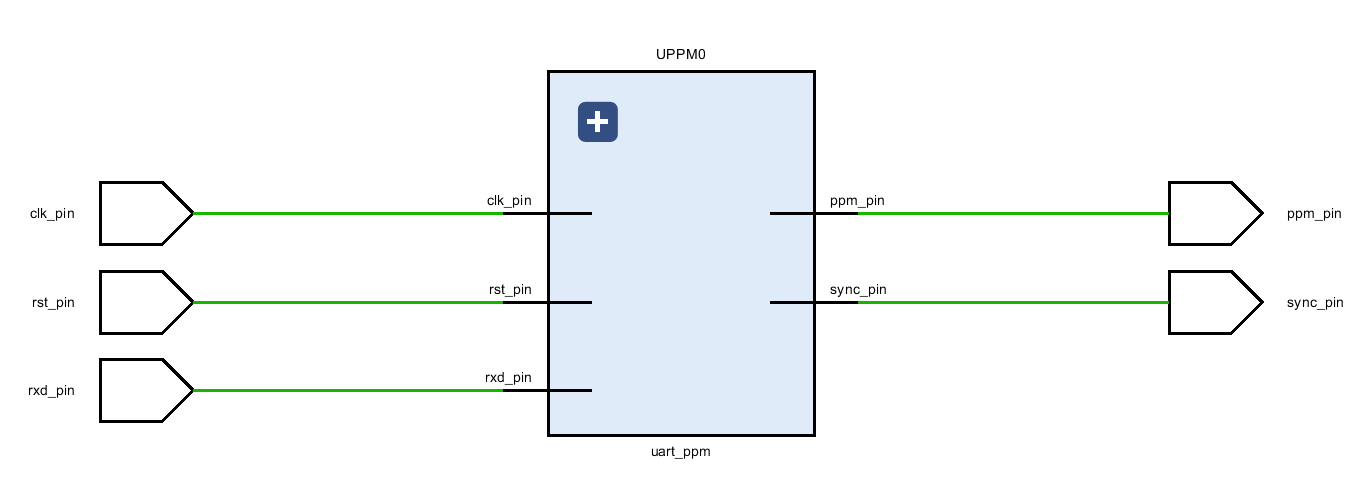
\includegraphics[width=0.85\linewidth]{fig/img1_bloque_ppm.png}
  \caption{Esquem\'atico de Vivado: nivel superior (\code{uart_top}), con \code{uart_ppm} como caja negra.}
  \label{fig:esqtop}
\end{figure}

\begin{figure}[H]
  \centering
  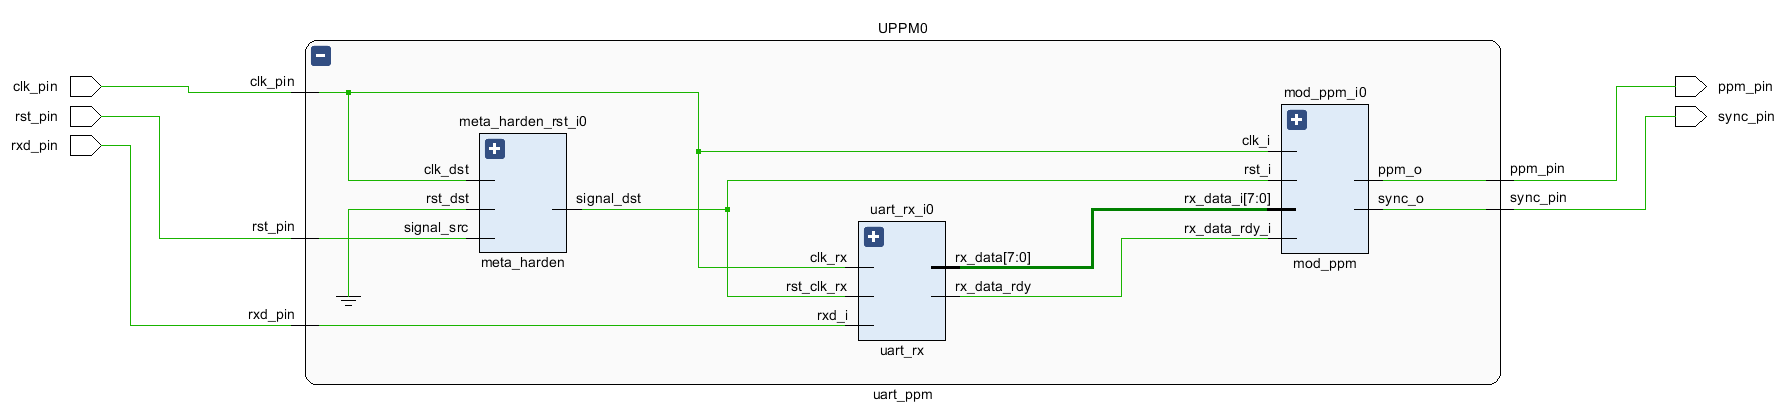
\includegraphics[width=\linewidth]{fig/img2_bloques_ppm.png}
  \caption{Esquem\'atico de Vivado: interior de \code{uart_ppm}, con \code{meta_harden}, \code{uart_rx} y \code{mod_ppm}.}
  \label{fig:esquart}
\end{figure}

\subsection{Temporización}

A \SI{125}{\mega\hertz} el diseño cumple la temporización (tabla~\ref{tab:timing} y figura~\ref{fig:vivadotiming}).

\begin{table}[H]
\centering
\small
\renewcommand{\arraystretch}{0.9}
\caption{Resumen de temporización después de la implementación (\SI{125}{\mega\hertz}).}
\label{tab:timing}
\begin{tabular}{@{}l r@{}}
\toprule
\textbf{Parámetro} & \textbf{Resultado} \\
\midrule
Worst Negative Slack (setup) & \SI{+3,908}{\nano\second} \\
Worst Hold Slack & \SI{+0,120}{\nano\second} \\
Worst Pulse Width Slack & \SI{+3,500}{\nano\second} \\
Endpoints analizados / que fallan & 168 / 0 \\
\bottomrule
\end{tabular}
\end{table}

\begin{figure}[H]
  \centering
  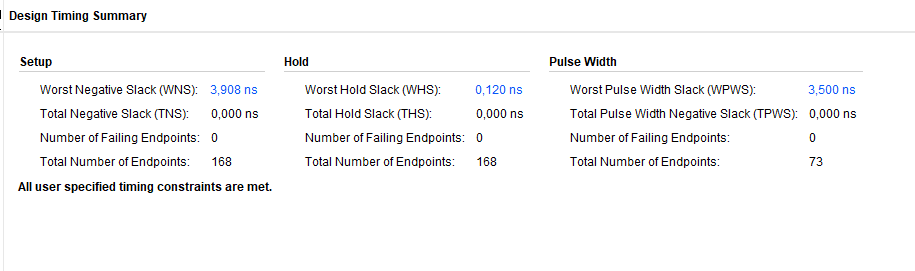
\includegraphics[width=0.8\linewidth]{fig/vivado_timing.png}
  \caption{\emph{Design Timing Summary} del diseño implementado.}
  \label{fig:vivadotiming}
\end{figure}



\subsection{Uso de recursos}

Las tablas~\ref{tab:recursos} y~\ref{tab:recmod} y la figura~\ref{fig:vivadoutil} muestran el uso de recursos de la FPGA, en total y por módulo.

\noindent
\begin{minipage}[t]{0.50\linewidth}
\centering
\footnotesize
\setlength{\tabcolsep}{3pt}
\renewcommand{\arraystretch}{0.85}
\captionof{table}{Uso de recursos de la FPGA.}
\label{tab:recursos}
\begin{tabular}{@{}l r r r@{}}
\toprule
\textbf{Recurso} & \textbf{Utilizado} & \textbf{Disponible} & \textbf{Utilización} \\
\midrule
LUT & 66 & \num{17600} & \SI{0,38}{\percent} \\
Flip-flops & 72 & \num{35200} & \SI{0,20}{\percent} \\
Entradas/salidas & 5 & 100 & \SI{5,00}{\percent} \\
BRAM / DSP & 0 & -- & \SI{0}{\percent} \\
\bottomrule
\end{tabular}
\end{minipage}\hfill
\begin{minipage}[t]{0.48\linewidth}
\centering
\footnotesize
\setlength{\tabcolsep}{3pt}
\renewcommand{\arraystretch}{0.85}
\captionof{table}{Uso de recursos por módulo.}
\label{tab:recmod}
\begin{tabular}{@{}l r r@{}}
\toprule
\textbf{Módulo} & \textbf{LUTs} & \textbf{Flip-flops} \\
\midrule
\code{uart_top} (total) & 66 & 72 \\
\quad \code{mod_ppm} & 30 & 40 \\
\quad \code{uart_rx} & 36 & 30 \\
\qquad \code{uart_rx_ctl} & 28 & 20 \\
\qquad \code{uart_baud_gen} & 8 & 8 \\
\qquad \code{meta_harden} (rxd) & 0 & 2 \\
\quad \code{meta_harden} (reset) & 0 & 2 \\
\bottomrule
\end{tabular}
\end{minipage}

\begin{figure}[H]
  \centering
  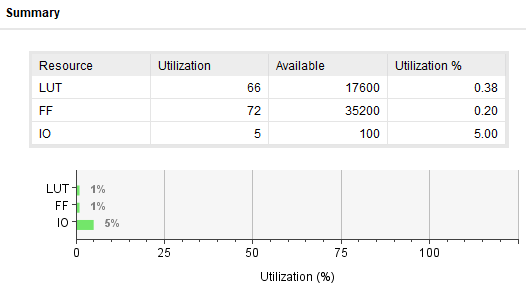
\includegraphics[width=0.55\linewidth]{fig/vivado_util.png}
  \caption{Resumen de utilización de Vivado.}
  \label{fig:vivadoutil}
\end{figure}


% =============================== 7. HARDWARE ===============================
\section{Verificación en hardware}

Se generó el bitstream y se programó la placa con Vivado. Luego, se realizó el montaje de los elementos para observar la salida de la FPGA.

\subsection{Montaje}

En la tabla~\ref{tab:conex} se especifica la conexión a la FPGA del analizador lógico y del adaptador USB-serie, y en la figura~\ref{fig:banco} se muestra el montaje.

\begin{table}[H]
\centering
\small
\renewcommand{\arraystretch}{0.9}
\caption{Conexiones al conector PMOD JA.}
\label{tab:conex}
\begin{tabular}{@{}l l@{}}
\toprule
\textbf{Desde} & \textbf{Hacia (PMOD JA)} \\
\midrule
Adaptador USB-serie, TxD & pin 1 (\code{rxd_pin}) \\
Adaptador USB-serie, GND & pin 5 (GND) \\
Analizador lógico, canal PPM\_OUTPUT & pin 3 (\code{ppm_pin}) \\
Analizador lógico, canal SYNC\_OUTPUT & pin 4 (\code{sync_pin}) \\
Analizador lógico, GND & pin 11 (GND) \\
\bottomrule
\end{tabular}
\end{table}

\begin{figure}[H]
  \centering
  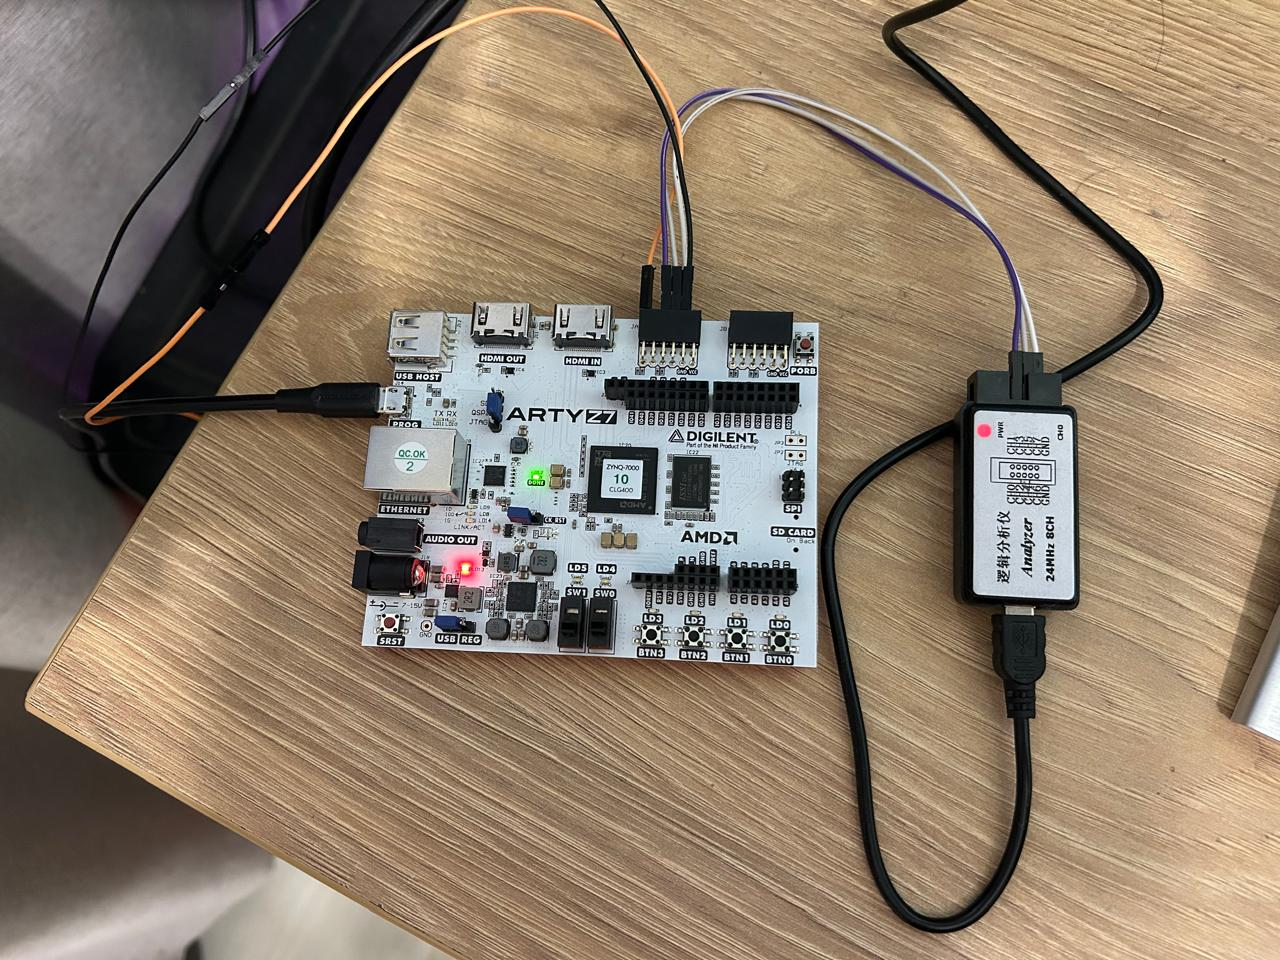
\includegraphics[width=0.6\linewidth]{fig/banco.jpeg}
  \caption{Montaje de prueba: placa Arty Z7-10 configurada, con el adaptador USB-serie y el analizador lógico conectados al conector PMOD JA.}
  \label{fig:banco}
\end{figure}

Los caracteres se enviaron desde un terminal serie (PuTTY) por el adaptador USB-serie a \num{115200} baudios, 8N1. El analizador lógico muestreó a \SI{24}{\mega\hertz}.

\subsection{Mediciones}

En esta sección se detallan las mediciones efectuadas con el analizador lógico y las capturas.

\subsubsection{Período entre pulsos de sincronización}

Se capturó \code{sync_pin} y se midió el tiempo entre dos flancos de subida consecutivos (figura~\ref{fig:hwperiodo}). El resultado fue de \SIrange{2,559}{2,560}{\milli\second}, que coincide prácticamente con los \SI{2,56}{\milli\second} esperados y confirma el funcionamiento de los contadores y del clock.

\begin{figure}[H]
  \centering
  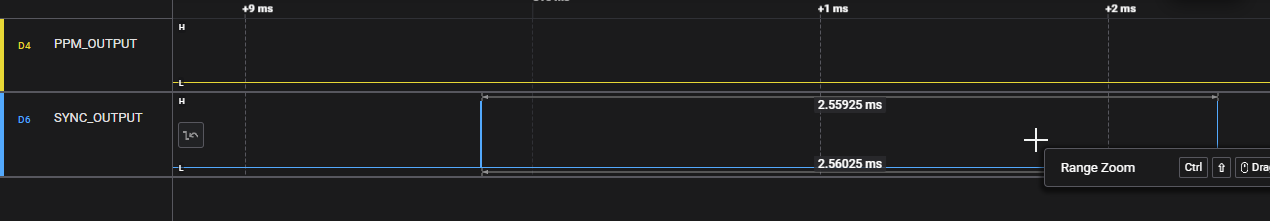
\includegraphics[width=\linewidth]{fig/hw_periodo.png}
  \caption{Período entre pulsos de \code{sync_pin}: \SI{2,56}{\milli\second}.}
  \label{fig:hwperiodo}
\end{figure}

\subsubsection{Ancho de pulso de sincronización}

Con un zoom sobre un solo pulso de \code{sync_pin} se midió su ancho (figura~\ref{fig:hwsync}), que resultó de
\SI{1}{\micro\second}. Es el valor esperado, ya que equivale a los 125 ciclos de \code{W_SYNC} a
\SI{125}{\mega\hertz}.

\begin{figure}[H]
  \centering
  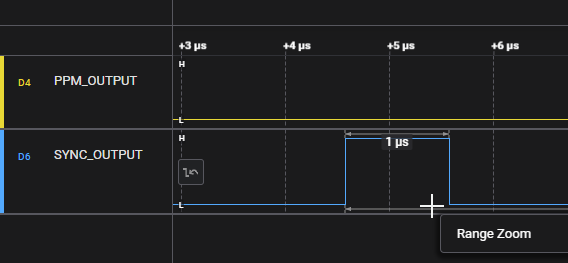
\includegraphics[width=0.75\linewidth]{fig/hw_sync_1us.png}
  \caption{Ancho del pulso de \code{sync_pin}: \SI{1}{\micro\second}.}
  \label{fig:hwsync}
\end{figure}

\subsubsection{Ancho de pulso de dato}

Del mismo modo se midió el ancho de un pulso de \code{ppm_pin} (figura~\ref{fig:hwppm}): \SI{10}{\micro\second},
exactamente una ranura (1250 ciclos), como corresponde al diseño.

\begin{figure}[H]
  \centering
  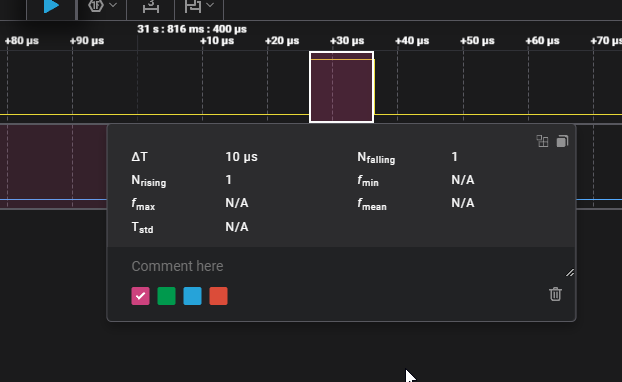
\includegraphics[width=0.6\linewidth]{fig/hw_ppm_10us.png}
  \caption{Ancho del pulso de \code{ppm_pin}: \SI{10}{\micro\second}.}
  \label{fig:hwppm}
\end{figure}

\subsubsection{Envío de datos}

Se enviaron caracteres desde el terminal serie y se midió, con dos marcadores, el tiempo entre el flanco de
subida de \code{sync_pin} y el de \code{ppm_pin}. Para la \texttt{'A'} (65) el retardo fue de
\SI{649,785}{\micro\second} (figura~\ref{fig:hwA}), frente a los \SI{650}{\micro\second} esperados. Con otros tres
caracteres (figura~\ref{fig:hwretardos}) se obtuvieron \SI{320,011}{\micro\second} para el byte 32,
\SI{480,056}{\micro\second} para el \texttt{'0'} y \SI{490,062}{\micro\second} para el \texttt{'1'}. En todos los
casos el retardo coincide con $d \times \SI{10}{\micro\second}$, y la diferencia entre el \texttt{'0'} y el
\texttt{'1'} es de una ranura (\SI{10}{\micro\second}), lo que verifica la resolución del sistema.

\begin{figure}[H]
  \centering
  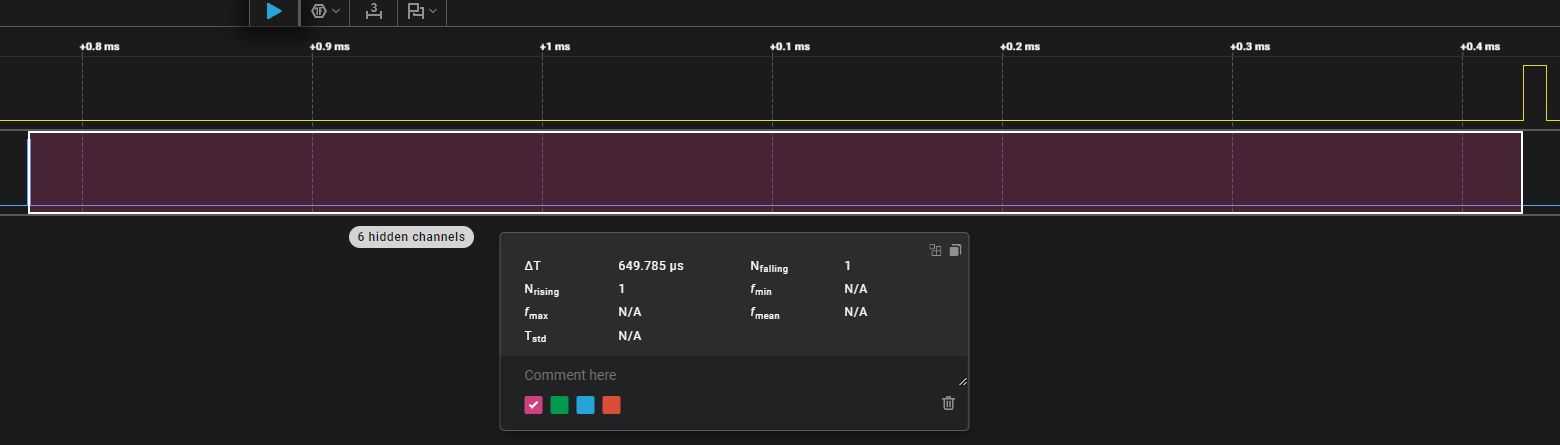
\includegraphics[width=\linewidth]{fig/hw_A_650us.png}
  \caption{Carácter \texttt{'A'} (ASCII 65): el pulso de \code{ppm_pin} aparece \SI{649,785}{\micro\second} después del sync.}
  \label{fig:hwA}
\end{figure}

\begin{figure}[H]
  \centering
  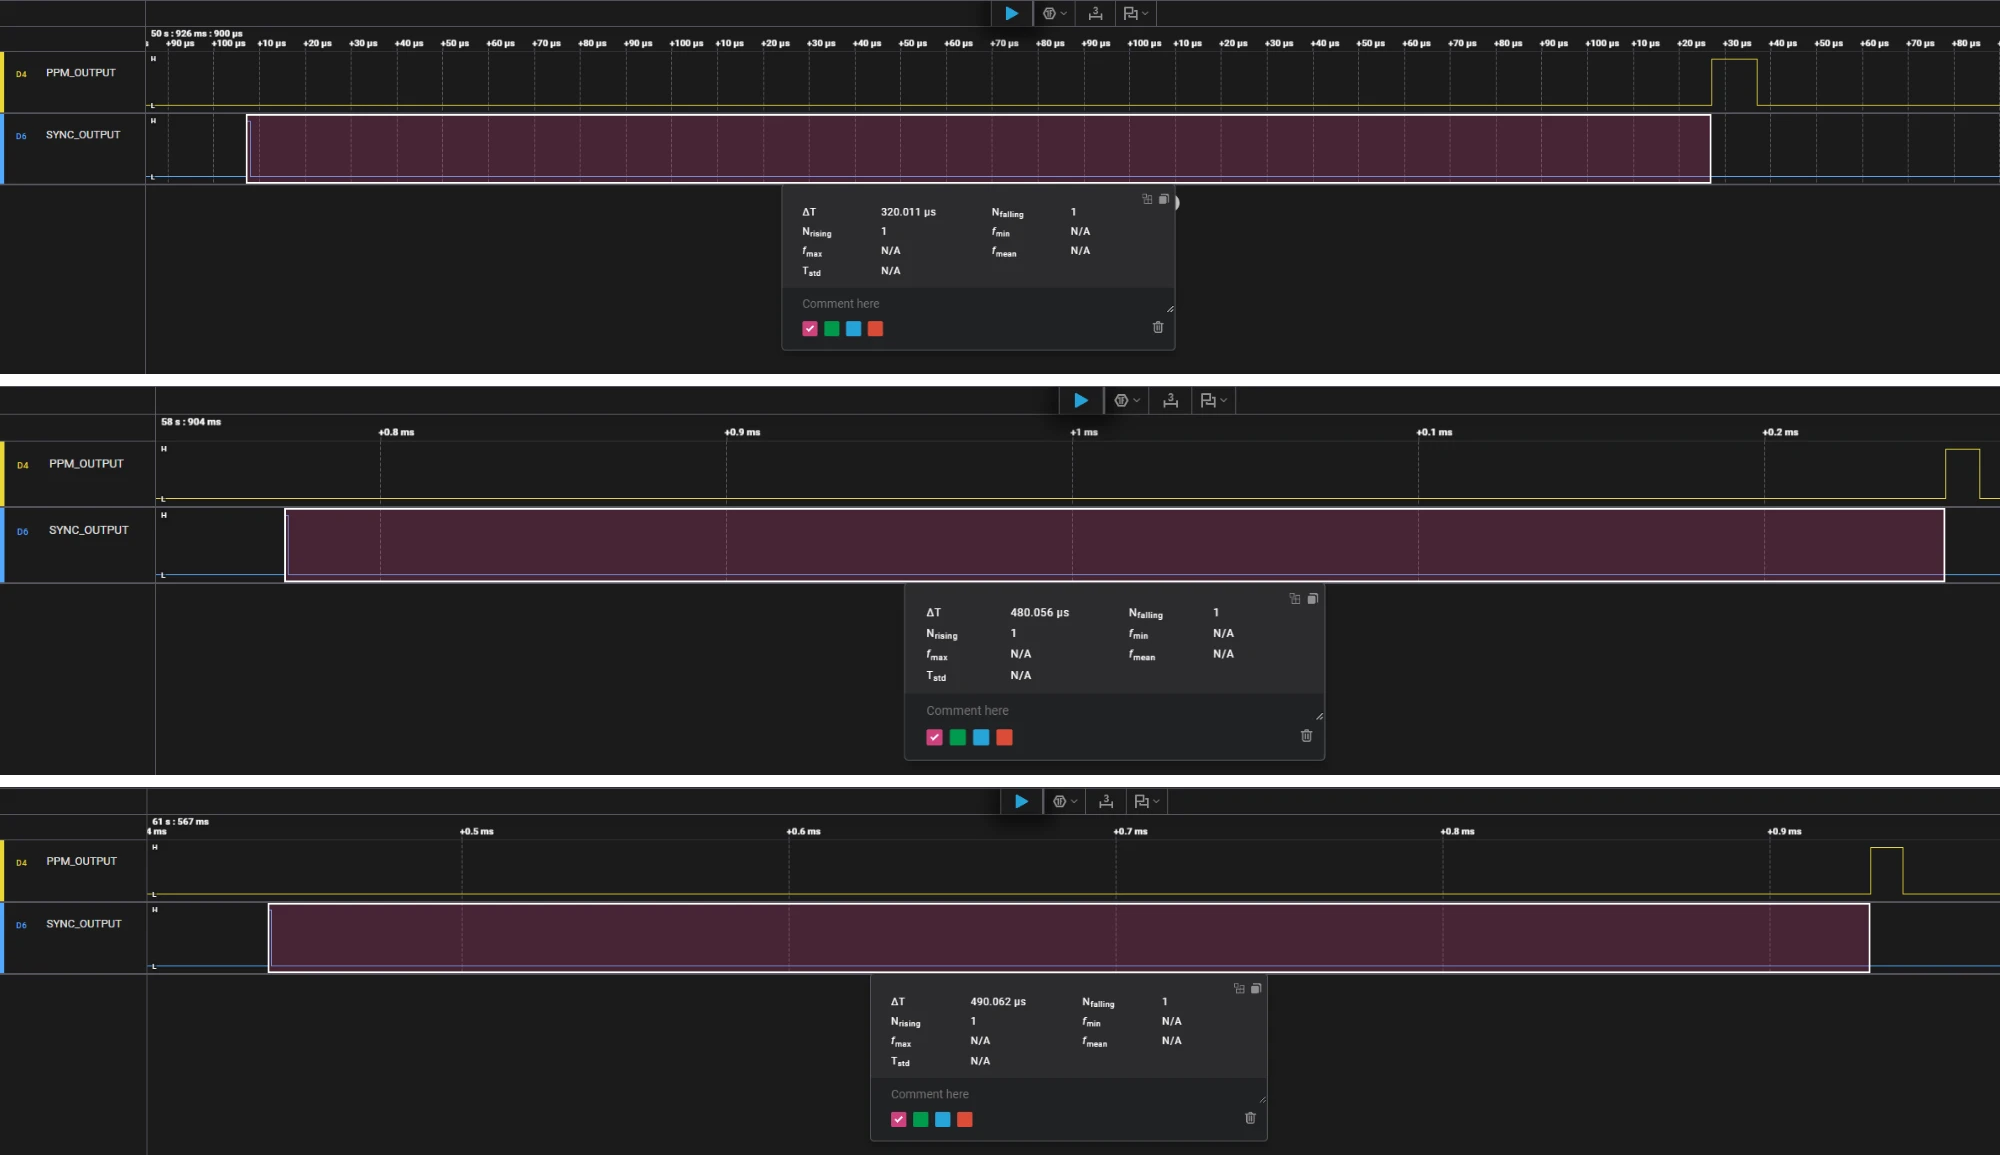
\includegraphics[width=\linewidth]{fig/hw_retardos.png}
  \caption{Retardo entre \code{sync_pin} y \code{ppm_pin} para tres caracteres: byte 32 (\SI{320}{\micro\second}), \texttt{'0'} (\SI{480}{\micro\second}) y \texttt{'1'} (\SI{490}{\micro\second}).}
  \label{fig:hwretardos}
\end{figure}

\subsubsection{Resumen de mediciones}

La tabla~\ref{tab:medidas} reúne las mediciones y las compara con los valores esperados.

\begin{table}[H]
\centering
\small
\renewcommand{\arraystretch}{0.9}
\caption{Mediciones con el analizador lógico.}
\label{tab:medidas}
\begin{tabular}{@{}l r r@{}}
\toprule
\textbf{Medición} & \textbf{Esperado} & \textbf{Medido} \\
\midrule
Período de \code{sync_pin} & \SI{2,56}{\milli\second} & \SIrange{2,559}{2,560}{\milli\second} \\
Ancho del pulso de \code{sync_pin} & \SI{1}{\micro\second} & \SI{1}{\micro\second} \\
Ancho del pulso de \code{ppm_pin} & \SI{10}{\micro\second} & \SI{10}{\micro\second} \\
Retardo sync-ppm, byte 32 (barra espaciadora) & \SI{320}{\micro\second} & \SI{320,011}{\micro\second} \\
Retardo sync-ppm, \texttt{'0'} (48) & \SI{480}{\micro\second} & \SI{480,056}{\micro\second} \\
Retardo sync-ppm, \texttt{'1'} (49) & \SI{490}{\micro\second} & \SI{490,062}{\micro\second} \\
Retardo sync-ppm, \texttt{'A'} (65) & \SI{650}{\micro\second} & \SI{649,785}{\micro\second} \\
\bottomrule
\end{tabular}
\end{table}

Las diferencias son menores que \SI{0,25}{\micro\second}, es decir, menos del \SI{2,5}{\percent} de una ranura.

\subsection{Prueba del reset}

Con el sistema funcionando se mantuvo presionado el botón de reset (BTN3) durante distintos intervalos. Mientras el botón está presionado, \code{sync_pin} queda en bajo y no se genera ningún pulso en \code{ppm_pin}; al soltarlo,
\code{sync_pin} retoma de inmediato con una trama nueva. Las ráfagas de pulsos de \code{ppm_pin} coinciden con los
caracteres tecleados y ninguna cae dentro de un reset.

\begin{figure}[H]
  \centering
  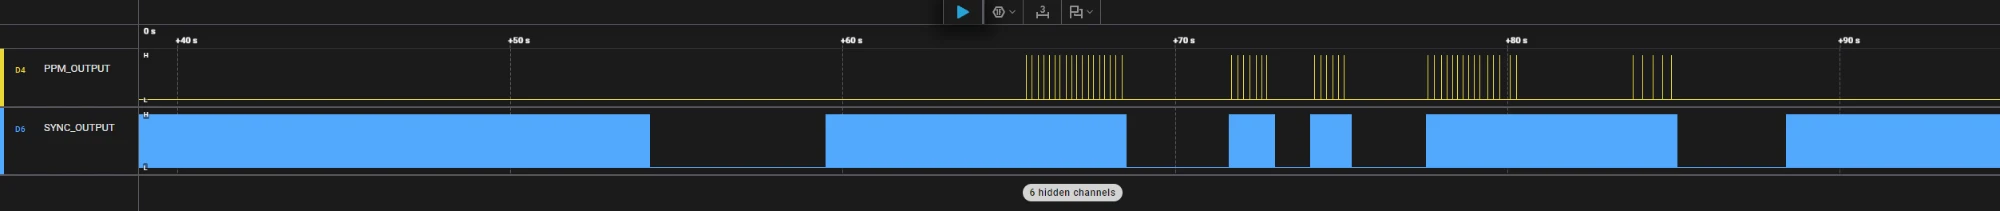
\includegraphics[width=\linewidth]{fig/hw_reset.png}
  \caption{Prueba del reset (escala de segundos): los huecos de \code{sync_pin} son los intervalos con BTN3 apretado.}
  \label{fig:hwreset}
\end{figure}

% =============================== 8. CONCLUSIONES ===============================
\section{Conclusiones}

Se implementó en la Arty Z7-10 un modulador PPM que convierte cada byte recibido por UART en la posición de un
pulso dentro de una trama de \SI{2,56}{\milli\second}, con una salida de sincronismo para medirla. El diseño
ocupa muy pocos recursos de la FPGA, cumple la temporización a \SI{125}{\mega\hertz} con
\SI{3,9}{\nano\second} de margen, y las mediciones en hardware coinciden con los valores teóricos con diferencias menores que \SI{0,25}{\micro\second}.
\end{document}
